\documentclass[11pt,a4paper]{article}

% Basic packages
\usepackage[utf8]{inputenc}
\usepackage[T1]{fontenc}
\usepackage{lmodern}
\usepackage[margin=2.5cm]{geometry}
\usepackage{amsmath,amssymb,amsfonts}
\usepackage{amsthm}
\usepackage{booktabs}
\usepackage{multirow}
\usepackage{array}
\usepackage{graphicx}
\usepackage{xcolor}
\usepackage{hyperref}
\usepackage[natbib=true,backend=biber,style=authoryear]{biblatex}
\addbibresource{references.bib}
\usepackage{algorithm}
\usepackage{algpseudocode}
\usepackage{caption}
\usepackage{subcaption}
\usepackage{enumitem}
\usepackage{appendix}

% TikZ & PGFPlots
\usepackage{tikz}
\usepackage{pgfplots}
\pgfplotsset{compat=1.18}
\usetikzlibrary{shapes,arrows,positioning,fit,calc,backgrounds,patterns,decorations.pathreplacing,matrix,shapes.multipart}
\usetikzlibrary{pgfplots.statistics,pgfplots.colorbrewer}

% Theorem environments
\newtheorem{definition}{Definition}
\newtheorem{theorem}{Theorem}
\newtheorem{lemma}{Lemma}
\newtheorem{proposition}{Proposition}

% Math operators
\DeclareMathOperator*{\argmin}{arg\,min}
\DeclareMathOperator*{\argmax}{arg\,max}
\DeclareMathOperator{\sign}{sign}
\DeclareMathOperator{\popcnt}{popcnt}
\DeclareMathOperator{\Hamming}{Hamming}
\DeclareMathOperator{\E}{\mathbb{E}}
\DeclareMathOperator{\Var}{Var}

% Colors
\definecolor{darkblue}{RGB}{0,51,102}
\definecolor{myblue}{RGB}{51,102,204}
\definecolor{myorange}{RGB}{230,126,34}
\definecolor{mygreen}{RGB}{39,174,96}
\definecolor{myred}{RGB}{231,76,60}
\definecolor{mypurple}{RGB}{142,68,173}
\definecolor{myteal}{RGB}{22,160,133}
\hypersetup{
    colorlinks=true,
    linkcolor=darkblue,
    citecolor=darkblue,
    urlcolor=darkblue,
}

\title{
\textbf{HSH-64: A 64-bit Learned Semantic Hashing Scheme}\\
\textbf{for Lightweight Semantic Retrieval}
}

\author{
  Zhihao Wu \\
  \texttt{1938258545@qq.com}
}

\date{\today}

\begin{document}

\maketitle

\begin{abstract}
Semantic hashing maps high-dimensional continuous embeddings into compact binary codes, enabling sub-linear approximate nearest neighbor (ANN) search with minimal memory footprint. However, conventional hashing methods often suffer from a large recall gap compared with brute-force embedding retrieval, especially when the code length is constrained for edge deployment. In this work, we present \textbf{HSH-64}, a 64-bit learned semantic hashing scheme specifically designed for lightweight Chinese vocabulary-level semantic retrieval. HSH-64 adopts a structured code format of \texttt{feat(4) + sim(52) + abs(8)} bits, where the 52-bit semantic similarity code is learned end-to-end through a three-stage pipeline: (1) continuous pre-training with a strong teacher model, (2) discrete fine-tuning with straight-through estimators (STE), and (3) recall-oriented post-processing via greedy bit-flip optimization. To reduce the online search cost, we further integrate Multi-Index Hashing (MIH) with adaptive radius expansion, asymmetric distance scoring, and a two-stage retrieval architecture that uses a lightweight encoder for coarse ranking and a stronger model for re-ranking. Extensive experiments on a 3,109-word Chinese vocabulary show that the best single Deep Hash model (h512, 1.17 MB) achieves Recall@10 of \textbf{0.7404} in pure Hamming space, while the lightweight variant (h256, 585 KB) reaches \textbf{0.7382}. A small ensemble of four models reaches \textbf{0.7724}. With MIH coarse ranking followed by a bge-large re-ranker, the four-model-ensemble two-stage system attains Recall@10 of \textbf{0.8970}. The source code and reproducible scripts are available at \url{https://github.com/Sauomore/Cabinet_hsh64}.
\end{abstract}

% ======================================================================
\section{Introduction}
% ======================================================================

Approximate nearest neighbor (ANN) search in high-dimensional embedding spaces is a fundamental building block for modern information retrieval, recommendation systems, and large language model augmentation \citep{jegou2011product,guo2020deep}. Dense retrieval based on pre-trained language models such as BERT \citep{devlin2019bert} and sentence-transformers \citep{reimers2019sentence} has achieved remarkable accuracy, yet brute-force comparison of floating-point vectors is prohibitively expensive for large corpora or latency-sensitive edge devices.

Semantic hashing \citep{salakhutdinov2009semantic} offers an attractive alternative: it compresses each vector into a short binary code so that similarity can be approximated by fast bit operations, e.g., Hamming distance via CPU \texttt{POPCNT}. Early methods relied on linear projections such as PCA or spectral hashing \citep{weiss2009spectral}; more recent deep hashing approaches \citep{xia2014supervised,cao2015deep,li2016feature} train neural networks end-to-end to produce binary codes that preserve semantic neighborhood structure. Despite progress, two practical challenges remain:
\begin{enumerate}[leftmargin=*]
    \item \textbf{Recall--efficiency trade-off.} Short codes reduce storage and computation but have limited information capacity, leading to lower recall compared with full embeddings.
    \item \textbf{Deployment cost.} State-of-the-art retrieval often depends on large encoder models (e.g., bge-large) at inference time, which is unsuitable for lightweight devices.
\end{enumerate}

In this paper, we tackle both challenges by introducing HSH-64 (\textbf{H}ierarchical \textbf{S}emantic \textbf{H}ashing), a 64-bit learned semantic hashing scheme. The key insight is that semantic hashing for vocabulary-level retrieval can exploit three structural properties: (i) items can be coarsely partitioned by part-of-speech or semantic category, (ii) the core semantic similarity signal can be captured by a moderate number of binary hyperplanes, and (iii) items within the same coarse cluster can be efficiently disambiguated by a short perfect-hash identifier. Our contributions are:
\begin{itemize}[leftmargin=*]
    \item We propose a structured 64-bit code, \texttt{feat(4) + sim(52) + abs(8)}, that separates part-of-speech features, semantic similarity bits, and intra-cluster perfect-hash identifiers. The design is hardware-friendly (single 64-bit integer, one \texttt{POPCNT}) and interpretable.
    \item We design a \textbf{three-stage training pipeline}---continuous pre-training, discrete fine-tuning with STE, and recall-oriented greedy post-processing---that significantly improves the quality of the 52-bit semantic code.
    \item We equip HSH-64 with an \textbf{adaptive Multi-Index Hashing (MIH)} coarse ranker, asymmetric distance scoring, and a two-stage retrieval architecture that uses a small encoder online while leveraging a stronger model only during training or optional re-ranking.
    \item We provide an extensive empirical study on a 3,109-word Chinese vocabulary benchmark, including model-capacity analysis, post-processing hyper-parameter search, ensemble strategy comparison, and efficiency benchmarks. A single lightweight model (585 KB) achieves 0.7382 Recall@10 in pure Hamming space, the best single post-processed model (1.17 MB) reaches 0.7404, an ensemble reaches 0.7724, and the full two-stage system reaches 0.8970 Recall@10.
\end{itemize}

% ======================================================================
\section{Related Work}
% ======================================================================

\subsection{Semantic Hashing}

Early unsupervised methods such as Locality-Sensitive Hashing (LSH) \citep{datar2004locality} and Spectral Hashing \citep{weiss2009spectral} construct binary codes via random projections or spectral decomposition of similarity graphs. The key limitation of LSH is that random hyperplanes do not exploit the semantic structure of the embedding space, leading to suboptimal recall for a given code length. Supervised hashing \citep{liu2012supervised,shen2015supervised} incorporates label information to improve discrimination. Deep hashing \citep{xia2014supervised,cao2015deep} uses neural networks to directly map raw inputs or embeddings to binary codes, often optimizing pairwise similarity-preserving losses. Our work extends this line by introducing a structured multi-field code and a three-stage training pipeline that specifically targets recall-oriented optimization.

\subsection{Straight-Through Estimators for Discrete Optimization}

Because the sign/quantization function has zero gradient almost everywhere, training deep hashers requires gradient estimators. The straight-through estimator (STE) \citep{bengio2013estimating} copies gradients through the sign function and is widely used in binary neural networks and hashing \citep{courbariaux2016binarized}. We employ STE in Stage 2 of our pipeline and complement it with a post-processing stage that directly optimizes the discrete codes without gradient approximation.

\subsection{Multi-Index Hashing}

MIH \citep{norouzi2012fast} splits a long binary code into multiple substrings and builds inverted indices for each substring. Given a query, it enumerates substrings within a small Hamming radius and merges candidates. Adaptive radius expansion balances recall and candidate pool size \citep{wang2018survey}. We adopt MIH with a novel adaptive stopping criterion that dynamically determines the search radius based on candidate pool saturation.

\subsection{Product Quantization and Compact Codes}

Product Quantization (PQ) \citep{jegou2011product} decomposes the vector space into a Cartesian product of low-dimensional subspaces and quantizes each subspace independently. For a 64-bit budget, PQ typically uses 8 subspaces of 8 bits each, requiring a learned codebook per subspace. Compared with HSH-64, PQ offers higher recall in many settings but at the cost of storing full-resolution codebooks and computing exact distances in the candidate re-ranking phase. HSH-64 trades some recall for extreme storage efficiency (8 bytes per item) and hardware-accelerated comparison via \texttt{POPCNT}.

\subsection{Knowledge Distillation for Retrieval}

Distilling a large teacher model into a compact student is common for efficient retrieval \citep{hinton2015distilling,izacard2020distilling}. We apply this idea twice: first, distilling bge-large teacher embeddings into a small MLP projector; second, distilling strong HSH codes into a lightweight student that only needs bge-small inputs at deployment.

% ======================================================================
\section{Problem Formulation}
% ======================================================================

Let $\mathcal{X} = \{\mathbf{x}_1, \dots, \mathbf{x}_N\}$ be a vocabulary of $N$ items, each represented by a continuous embedding $\mathbf{x}_i \in \mathbb{R}^D$ produced by a lightweight encoder (e.g., bge-small). Let $\mathcal{T} = \{\mathbf{t}_1, \dots, \mathbf{t}_N\}$ be the corresponding teacher embeddings produced by a stronger model (e.g., bge-large). The cosine similarity between items $i$ and $j$ is
\begin{equation}
    s_{ij} = \frac{\mathbf{t}_i^\top \mathbf{t}_j}{\| \mathbf{t}_i \| \| \mathbf{t}_j \|}.
\end{equation}
The ground-truth top-$K$ neighbor set for item $i$ is
\begin{equation}
    \mathcal{G}_i^{(K)} = \argmax_{\mathcal{J} \subseteq [N] \setminus \{i\}, |\mathcal{J}|=K} \sum_{j \in \mathcal{J}} s_{ij}.
\end{equation}

A semantic hashing function $h: \mathbb{R}^D \to \{0,1\}^M$ maps each embedding to an $M$-bit binary code. We focus on $M=52$ for the semantic part, wrapped in a 64-bit structured code. The retrieval function returns the top-$K$ items with smallest Hamming distance:
\begin{equation}
    \mathcal{R}_i^{(K)} = \argmin_{\mathcal{J} \subseteq [N] \setminus \{i\}, |\mathcal{J}|=K} \sum_{j \in \mathcal{J}} d_H\bigl(h(\mathbf{x}_i), h(\mathbf{x}_j)\bigr).
\end{equation}
The objective is to maximize Recall@$K$:
\begin{equation}
    \text{Recall@}K = \frac{1}{N} \sum_{i=1}^{N} \frac{| \mathcal{R}_i^{(K)} \cap \mathcal{G}_i^{(K)} |}{K}.
\end{equation}

% ======================================================================
\section{HSH-64 Code Structure}
% ======================================================================

An HSH-64 code is a 64-bit unsigned integer partitioned into three fields:
\begin{equation}
    c = \underbrace{(f_3 f_2 f_1 f_0)}_{\text{feat}: 4}
    \,\|\,
    \underbrace{(s_{51} \cdots s_1 s_0)}_{\text{sim}: 52}
    \,\|\,
    \underbrace{(a_7 \cdots a_1 a_0)}_{\text{abs}: 8},
\end{equation}
where $\|$ denotes bit concatenation. Figure~\ref{fig:code-structure} visualizes the bit layout and field semantics.

\begin{figure}[htbp]
\centering
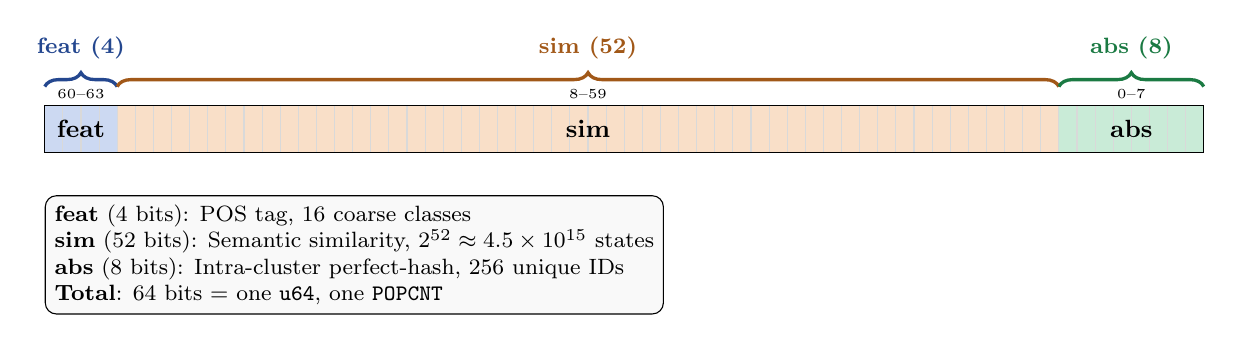
\begin{tikzpicture}[x=0.23cm, y=0.6cm,
    brace/.style={decorate, decoration={brace, amplitude=5pt}, very thick},
]
    % Horizontal bit strip: MSB (63) on left, LSB (0) on right
    \fill[myblue!25]   (0,0) rectangle (4,1);
    \fill[myorange!25] (4,0) rectangle (56,1);
    \fill[mygreen!25]  (56,0) rectangle (64,1);

    % Grid lines
    \foreach \i in {0,...,64} {
        \draw[gray!30] (\i,0) -- (\i,1);
    }
    \draw (0,0) rectangle (64,1);

    % Field labels
    \node[font=\small\bfseries] at (2,0.5) {feat};
    \node[font=\small\bfseries] at (30,0.5) {sim};
    \node[font=\small\bfseries] at (60,0.5) {abs};

    % Bit range labels
    \node[font=\tiny] at (2,1.25) {60--63};
    \node[font=\tiny] at (30,1.25) {8--59};
    \node[font=\tiny] at (60,1.25) {0--7};

    % Braces
    \draw[brace, myblue!70!black]   (0,1.4)  -- (4,1.4)  node[midway, above=6pt, font=\footnotesize\bfseries, text=myblue!70!black]   {feat (4)};
    \draw[brace, myorange!70!black] (4,1.4)  -- (56,1.4) node[midway, above=6pt, font=\footnotesize\bfseries, text=myorange!70!black] {sim (52)};
    \draw[brace, mygreen!70!black]  (56,1.4) -- (64,1.4) node[midway, above=6pt, font=\footnotesize\bfseries, text=mygreen!70!black]  {abs (8)};

    % Legend box
    \node[draw, rounded corners, fill=gray!5, font=\footnotesize, align=left, anchor=north west] at (0,-0.9) {
        \textbf{feat} (4 bits): POS tag, 16 coarse classes \\
        \textbf{sim} (52 bits): Semantic similarity, $2^{52} \approx 4.5\times 10^{15}$ states \\
        \textbf{abs} (8 bits): Intra-cluster perfect-hash, 256 unique IDs \\
        \textbf{Total}: 64 bits = one \texttt{u64}, one \texttt{POPCNT}
    };
\end{tikzpicture}
\caption{HSH-64 bit layout. The 64-bit code partitions into three color-coded fields: feat (blue, 4 bits), sim (orange, 52 bits), and abs (green, 8 bits). The entire code fits in a single 64-bit CPU register, enabling single-instruction Hamming distance computation via \texttt{POPCNT}.}
\label{fig:code-structure}
\end{figure}

The Hamming distance between two codes $c$ and $c'$ is computed by a single hardware popcount over the full 64 bits:
\begin{equation}
    d_H(c, c') = \popcnt(c \oplus c').
\end{equation}

\paragraph{Role of the abs field.} Although Equation~(6) computes the Hamming distance over all 64 bits, the abs field is designed to act as a tie-breaker rather than a semantic similarity signal. Two words that share the same $(\text{feat}, \text{sim})$ prefix but differ only in abs differ by at most 8 bits, placing them in a tight Hamming neighborhood. Two words with different sim codes, by contrast, typically differ by many more bits. Thus, abs determines the intra-cluster rank but does not dominate cross-cluster semantic distance. The abs field can also be used as a hard filter: requiring exact $(\text{feat}, \text{sim})$ match before consulting abs turns the 8-bit field into a perfect-hash lookup within each bucket.

\subsection{Information-Theoretic Preview}

The 52-bit sim code can represent up to $2^{52} \approx 4.5 \times 10^{15}$ distinct values---far more than the $N=3{,}109$ vocabulary items. A rigorous information-theoretic analysis, including Hamming ball capacity, Gilbert-Varshamov bounds, and expected distance distributions, is provided in Section~\ref{sec:math-analysis}.

Figure~\ref{fig:hamming-dist} illustrates the empirical effect of our optimization on Hamming distance distributions.

\begin{figure}[htbp]
\centering
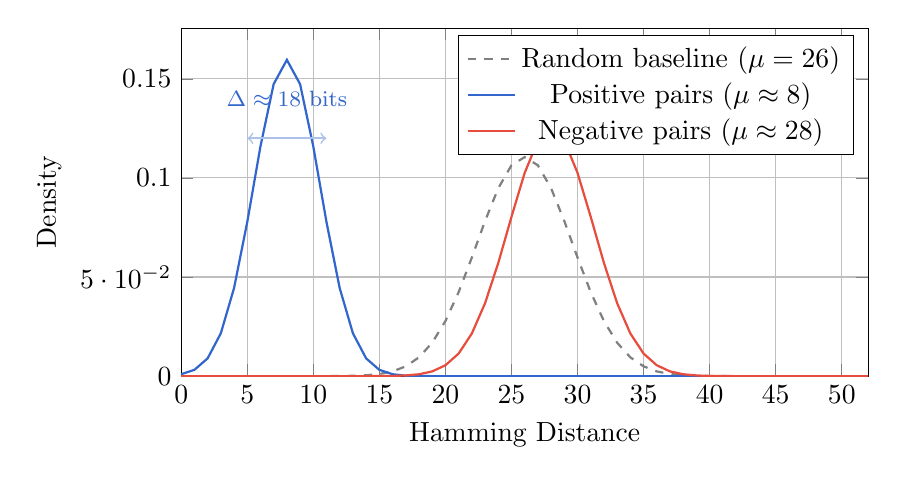
\begin{tikzpicture}
\begin{axis}[
    width=0.85\textwidth,
    height=6cm,
    xlabel={Hamming Distance},
    ylabel={Density},
    xmin=0, xmax=52,
    ymin=0,
    legend style={at={(0.98,0.98)}, anchor=north east},
    grid=major,
]
    % Random baseline
    \addplot[color=gray, thick, dashed, domain=0:52, samples=53]
        {1/(3.61*sqrt(2*pi)) * exp(-(x-26)^2/(2*3.61^2))};
    \addlegendentry{Random baseline ($\mu=26$)}

    % Positive pairs (after optimization) - approximate
    \addplot[color=myblue, thick, domain=0:52, samples=53]
        {1/(2.5*sqrt(2*pi)) * exp(-(x-8)^2/(2*2.5^2))};
    \addlegendentry{Positive pairs ($\mu\approx 8$)}

    % Negative pairs (after optimization) - approximate
    \addplot[color=myred, thick, domain=0:52, samples=53]
        {1/(3.2*sqrt(2*pi)) * exp(-(x-28)^2/(2*3.2^2))};
    \addlegendentry{Negative pairs ($\mu\approx 28$)}

    \draw[myblue!40, semithick, <->] (axis cs:5,0.12) -- (axis cs:11,0.12);
    \node[myblue, font=\footnotesize] at (axis cs:8,0.14) {$\Delta \approx 18$ bits};
\end{axis}
\end{tikzpicture}
\caption{Approximate Hamming distance distributions before and after optimization. The random baseline (dashed) centers at 26 bits. Post-optimization, positive pairs (blue) shift to a mean of $\sim$8 bits, while negative pairs (red) shift slightly above the random baseline, creating a separation of $\sim$18 bits.}
\label{fig:hamming-dist}
\end{figure}

% ======================================================================
\section{Methodology}
% ======================================================================

\subsection{Deep Hash MLP Architecture}\label{sec:mlp-arch}

Let $\mathbf{x} \in \mathbb{R}^D$ be a continuous embedding (e.g., from bge-small, $D=512$). We learn a multi-layer perceptron (MLP) that maps $\mathbf{x}$ to a continuous logit vector $\mathbf{u}$:
\begin{equation}
    \mathbf{u} = f_\theta(\mathbf{x} - \boldsymbol{\mu}),
\end{equation}
where $\boldsymbol{\mu}$ is the training-set mean. The binary semantic code is obtained by sign quantization:
\begin{equation}
    \mathbf{b} = \frac{1 + \sign(\mathbf{u})}{2} \in \{0, 1\}^{52}.
\end{equation}
During back-propagation, the sign function is replaced by the identity STE:
\begin{equation}
    \frac{\partial \mathbf{b}}{\partial \mathbf{u}} \approx \mathbf{I}.
\end{equation}

The network architecture is a simple MLP with one hidden layer:
\begin{equation}
    f_\theta(\mathbf{x}) = \mathbf{W}_2 \, \sigma(\mathbf{W}_1 \mathbf{x} + \mathbf{h}_1) + \mathbf{h}_2,
\end{equation}
where $\sigma$ is ReLU, $\mathbf{W}_1 \in \mathbb{R}^{H \times D}$, $\mathbf{W}_2 \in \mathbb{R}^{O \times H}$, and $H$ is the hidden dimension. The output dimension $O$ is task-dependent: $O=52$ for the final hashing layer (Section~\ref{sec:stage2}) and $O=D_t=1024$ for continuous teacher distillation in Stage~1 (Section~\ref{sec:stage1}). Figure~\ref{fig:mlp-arch} shows the architecture with $O=52$.

\begin{figure}[htbp]
\centering
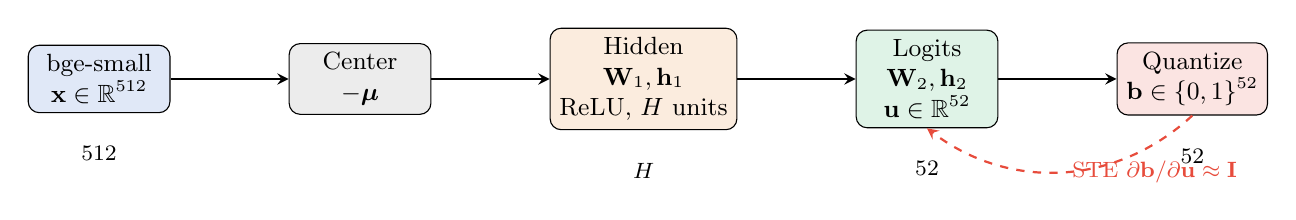
\begin{tikzpicture}[
    node distance=1.5cm,
    layer/.style={rectangle, draw, minimum width=1.8cm, minimum height=0.7cm, align=center, font=\small, rounded corners},
    arrow/.style={->, >=stealth, thick},
]
    % Input
    \node[layer, fill=myblue!15] (input) {bge-small\\$\mathbf{x} \in \mathbb{R}^{512}$};
    % Center
    \node[layer, fill=gray!15, right=of input] (center) {Center\\$-\boldsymbol{\mu}$};
    % Hidden
    \node[layer, fill=myorange!15, right=of center] (hidden) {Hidden\\$\mathbf{W}_1, \mathbf{h}_1$\\ReLU, $H$ units};
    % Output
    \node[layer, fill=mygreen!15, right=of hidden] (output) {Logits\\$\mathbf{W}_2, \mathbf{h}_2$\\$\mathbf{u} \in \mathbb{R}^{52}$};
    % Quantize
    \node[layer, fill=myred!15, right=of output] (quant) {Quantize\\$\mathbf{b} \in \{0,1\}^{52}$};

    \draw[arrow] (input) -- (center);
    \draw[arrow] (center) -- (hidden);
    \draw[arrow] (hidden) -- (output);
    \draw[arrow] (output) -- (quant);

    % Dimensions
    \node[font=\footnotesize, below=0.3cm of input] {$512$};
    \node[font=\footnotesize, below=0.3cm of hidden] {$H$};
    \node[font=\footnotesize, below=0.3cm of output] {$52$};
    \node[font=\footnotesize, below=0.3cm of quant] {$52$};

    % STE arrow
    \draw[arrow, myred, dashed, bend left=40] (quant.south) to node[font=\footnotesize, right, text=myred] {STE $\partial\mathbf{b}/\partial\mathbf{u} \approx \mathbf{I}$} (output.south);
\end{tikzpicture}
\caption{Deep Hash MLP architecture. The input embedding is centered, passed through a single hidden layer with ReLU, projected to 52 logits, and quantized to $\{0,1\}^{52}$ via sign. The dashed red arrow indicates the STE gradient path during training.}
\label{fig:mlp-arch}
\end{figure}

\subsection{Three-Stage Training Pipeline}

Figure~\ref{fig:pipeline} illustrates the complete three-stage training flow.

\begin{figure}[htbp]
\centering
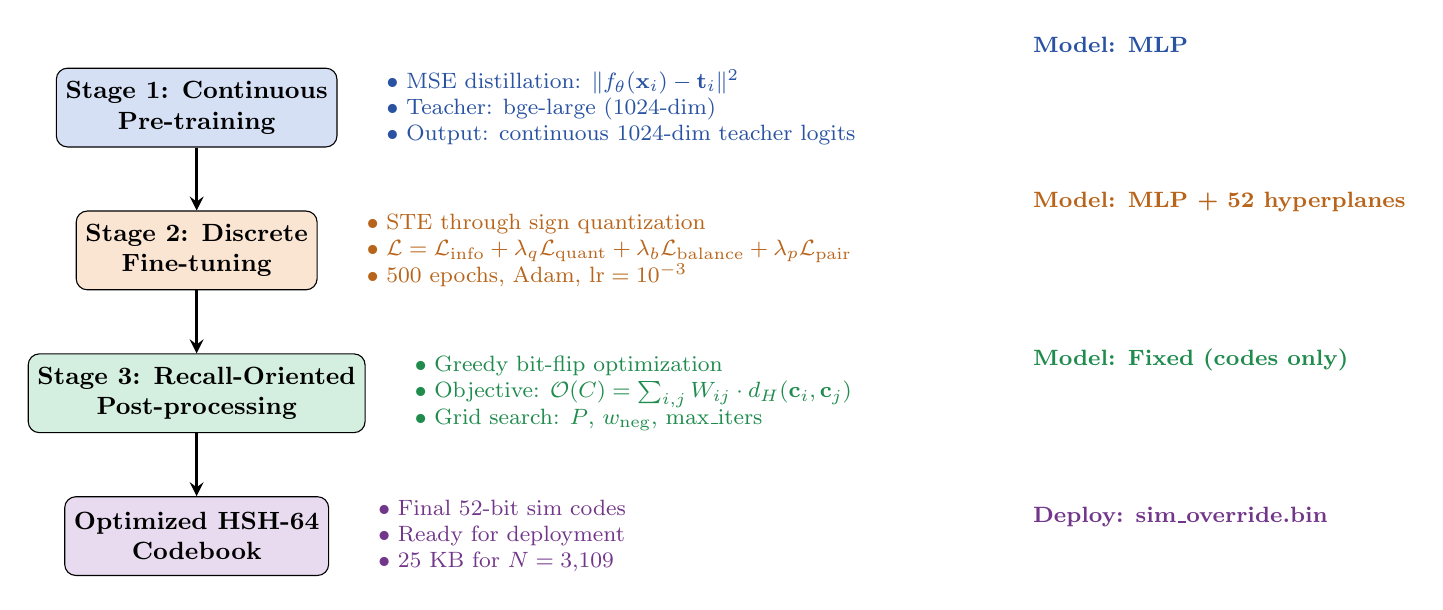
\begin{tikzpicture}[
    node distance=2.0cm and 1.0cm,
    block/.style={rectangle, draw, rounded corners, minimum width=3.0cm, minimum height=1.0cm, align=center, font=\small\bfseries, fill=#1!20},
    detail/.style={font=\footnotesize, align=left, text=#1!80!black},
    arrow/.style={->, >=stealth, very thick},
    sidearrow/.style={->, >=stealth, thick, draw=#1!60!black},
]
    % Stage 1
    \node[block={myblue}] (s1) {Stage 1: Continuous\\Pre-training};
    \node[detail={myblue}, right=0.5cm of s1] {
        $\bullet$ MSE distillation: $\|f_\theta(\mathbf{x}_i) - \mathbf{t}_i\|^2$ \\
        $\bullet$ Teacher: bge-large (1024-dim) \\
        $\bullet$ Output: continuous 1024-dim teacher logits
    };

    % Stage 2
    \node[block={myorange}, below=0.8cm of s1] (s2) {Stage 2: Discrete\\Fine-tuning};
    \node[detail={myorange}, right=0.5cm of s2] {
        $\bullet$ STE through sign quantization \\
        $\bullet$ $\mathcal{L} = \mathcal{L}_{\text{info}} + \lambda_q\mathcal{L}_{\text{quant}} + \lambda_b\mathcal{L}_{\text{balance}} + \lambda_p\mathcal{L}_{\text{pair}}$ \\
        $\bullet$ 500 epochs, Adam, $\text{lr}=10^{-3}$
    };

    % Stage 3
    \node[block={mygreen}, below=0.8cm of s2] (s3) {Stage 3: Recall-Oriented\\Post-processing};
    \node[detail={mygreen}, right=0.5cm of s3] {
        $\bullet$ Greedy bit-flip optimization \\
        $\bullet$ Objective: $\mathcal{O}(C) = \sum_{i,j} W_{ij} \cdot d_H(\mathbf{c}_i, \mathbf{c}_j)$ \\
        $\bullet$ Grid search: $P$, $w_{\text{neg}}$, max\_iters
    };

    % Output
    \node[block={mypurple}, below=0.8cm of s3] (out) {Optimized HSH-64\\Codebook};
    \node[detail={mypurple}, right=0.5cm of out] {
        $\bullet$ Final 52-bit sim codes \\
        $\bullet$ Ready for deployment \\
        $\bullet$ 25 KB for $N=3{,}109$
    };

    % Arrows
    \draw[arrow] (s1) -- (s2);
    \draw[arrow] (s2) -- (s3);
    \draw[arrow] (s3) -- (out);

    % Side annotations
    \node[font=\footnotesize\bfseries, myblue!80!black, anchor=west] at (10.5, 0.8) {Model: MLP};
    \node[font=\footnotesize\bfseries, myorange!80!black, anchor=west] at (10.5, -1.2) {Model: MLP + 52 hyperplanes};
    \node[font=\footnotesize\bfseries, mygreen!80!black, anchor=west] at (10.5, -3.2) {Model: Fixed (codes only)};
    \node[font=\footnotesize\bfseries, mypurple!80!black, anchor=west] at (10.5, -5.2) {Deploy: sim\_override.bin};
\end{tikzpicture}
\caption{The three-stage training pipeline of HSH-64. Stage 1 uses MSE distillation to provide a good continuous initialization. Stage 2 fine-tunes with STE and multi-objective loss. Stage 3 applies recall-oriented greedy bit-flip post-processing to directly optimize the final binary codes.}
\label{fig:pipeline}
\end{figure}

\subsubsection{Stage 1: Continuous Pre-training}\label{sec:stage1}

Stage~1 uses the same hidden layers as in Section~\ref{sec:mlp-arch}, but replaces the output layer with $D_t=1024$ units to match the bge-large teacher. Stage~2 then swaps the output layer back to 52 units, leveraging the Stage~1 continuous projection as initialization. Given a teacher model (bge-large) that produces high-quality embeddings $\mathbf{t} \in \mathbb{R}^{D_t}$, we first train the MLP to output continuous vectors that match the teacher:
\begin{equation}
    \mathcal{L}_{\text{MSE}} = \frac{1}{N} \sum_{i=1}^{N} \| f_\theta(\mathbf{x}_i) - \mathbf{t}_i \|_2^2.
\end{equation}
This stage provides a good initialization for the continuous projection. We train for 500 epochs with Adam at learning rate $10^{-3}$ on the full vocabulary.

\subsubsection{Stage 2: Discrete Fine-tuning}\label{sec:stage2}

We replace the Stage~1 output layer with a 52-hyperplane quantization layer and train end-to-end with the STE. The loss combines four terms:
\begin{align}
    \mathcal{L}_{\text{info}} &= -\frac{1}{|\mathcal{P}^+|}\sum_{(i,j) \in \mathcal{P}^+} \log \frac{e^{\mathbf{u}_i^\top \mathbf{u}_j / \tau}}{\sum_{k} e^{\mathbf{u}_i^\top \mathbf{u}_k / \tau}} \\
    \mathcal{L}_{\text{quant}} &= \frac{1}{N} \sum_{i=1}^{N} \| \mathbf{u}_i - \mathbf{b}_i \|_1 \\
    \mathcal{L}_{\text{balance}} &= \frac{1}{M} \sum_{j=1}^{M} \left( \bar{b}_j - 0.5 \right)^2 \\
    \mathcal{L}_{\text{pair}} &= \frac{1}{|\mathcal{P}|} \sum_{(i,j) \in \mathcal{P}} \left( \mathbf{u}_i^\top \mathbf{u}_j - \mathbf{t}_i^\top \mathbf{t}_j \right)^2,
\end{align}
where $\mathcal{P}^+$ is the set of positive pairs (top-$P$ teacher neighbors), $\mathcal{P}$ is a sampled set of pairs, $M=52$ is the code length, and $\bar{b}_j$ is the empirical mean of bit $j$ after sign quantization. The denominator in $\mathcal{L}_{\text{info}}$ traverses all $N$ vocabulary items (the batch size equals the full vocabulary). In computing $\mathcal{L}_{\text{pair}}$, both $\mathbf{u}_i$ and $\mathbf{t}_i$ are L2-normalized so that the inner products become cosine similarities. The total loss is
\begin{equation}
    \mathcal{L} = \mathcal{L}_{\text{info}} + \lambda_q \mathcal{L}_{\text{quant}} + \lambda_b \mathcal{L}_{\text{balance}} + \lambda_p \mathcal{L}_{\text{pair}}.
\end{equation}
In our implementation, $\lambda_q$ is initialized to 1.0 and linearly annealed to the configured target over the first 50\% of epochs; with the default target $\lambda_q=1.0$, the weight remains fixed. We use $\lambda_b=0.5$ and $\lambda_p=0.0$ by default.

\paragraph{Loss design rationale.} InfoNCE encourages the continuous logits to preserve the teacher's neighborhood structure. The quantization loss $\mathcal{L}_{\text{quant}}$ penalizes the discrepancy between continuous logits and their binarized counterparts, encouraging the network to produce confident, near-binary activations. The balance loss prevents bit collapse---the degenerate case where all items share the same bit value, wasting coding capacity. The pairwise loss directly aligns the inner-product structure of student logits with teacher embeddings, providing a fine-grained supervision signal.

\subsubsection{Stage 3: Recall-Oriented Post-processing}

After the MLP and hyperplanes are fixed, we optimize each binary code with a greedy bit-flip procedure whose objective directly targets Recall@$K$. Let $S \in \mathbb{R}^{N \times N}$ be the teacher cosine-similarity matrix and let $C \in \{0,1\}^{N \times M}$ be the current binary codes. For each query $i$, define the positive set $\mathcal{P}_i^+$ as the indices of the top-$P$ teacher neighbors, and the negative set $\mathcal{P}_i^-$ as words that are not in the positive set but currently appear in the Hamming top-$K$.

The recall-oriented weight for pair $(i,j)$ is
\begin{equation}
\label{eq:weight}
    W_{ij} =
    \begin{cases}
        +w_{\text{pos}}, & j \in \mathcal{P}_i^+ \\
        -w_{\text{neg}}, & j \in \mathcal{P}_i^- \\
        0, & \text{otherwise}.
\end{cases}
\end{equation}
The objective is
\begin{equation}
\label{eq:objective}
    \mathcal{O}(C) = \sum_{i,j} W_{ij} \cdot d_H(\mathbf{c}_i, \mathbf{c}_j),
\end{equation}
where $d_H$ is the Hamming distance. Minimizing $\mathcal{O}$ pulls positive neighbors closer and pushes hard negatives away in Hamming space. The greedy algorithm iteratively flips the bit that yields the largest reduction in $\mathcal{O}$ until convergence or a maximum number of iterations.

\begin{algorithm}[htbp]
\caption{Recall-oriented greedy bit-flip optimization.}
\label{alg:postprocess}
\begin{algorithmic}[1]
\Require Binary codes $C \in \{0,1\}^{N \times M}$, teacher similarity matrix $S$, positive count $P$, top-$K$, negative weight $w_{\text{neg}}$, max iterations $T$.
\Ensure Optimized codes $C$.
\State Compute positive sets $\mathcal{P}_i^+ \leftarrow \operatorname{top-\emph{P}}(S_i)$ for all $i$.
\For{$t = 1$ \textbf{to} $T$}
    \State Compute negative sets $\mathcal{P}_i^-$ from current Hamming top-$K$.
    \State Build weight matrix $W$ according to Eq.~(\ref{eq:weight}).
    \State Compute $\Delta_{i,b} = \mathcal{O}(C \text{ with bit } b \text{ of item } i \text{ flipped}) - \mathcal{O}(C)$.
    \State Find $(i^*, b^*) = \argmin_{i,b} \Delta_{i,b}$.
    \If{$\Delta_{i^*,b^*} < 0$}
        \State Flip $C_{i^*, b^*}$.
    \Else
        \State \textbf{break}.
    \EndIf
\EndFor
\State \Return $C$.
\end{algorithmic}
\end{algorithm}

\subsection{Asymmetric Distance Scoring}

Sign quantization discards the magnitude of the continuous projection. Asymmetric scoring mitigates this by using the query's continuous projection $\mathbf{u}_q$ and the database's quantized bits $\mathbf{b}_d$:
\begin{equation}
    s_{\text{asym}}(\mathbf{u}_q, \mathbf{b}_d) = \sum_{j=1}^{M} u_{q,j} \cdot (2 b_{d,j} - 1).
\end{equation}
Because the database bits are pre-computed, the online cost is one dot product per candidate. The asymmetric score provides a finer-grained ranking than Hamming distance by weighting each bit by the query's projection confidence.

\subsection{Multi-Index Hashing with Adaptive Radius}

For sub-linear retrieval, we split the 52-bit sim code into $B$ segments of equal length and build an inverted index for each segment. Figure~\ref{fig:mih-structure} illustrates the MIH segment structure.

\begin{figure}[htbp]
\centering
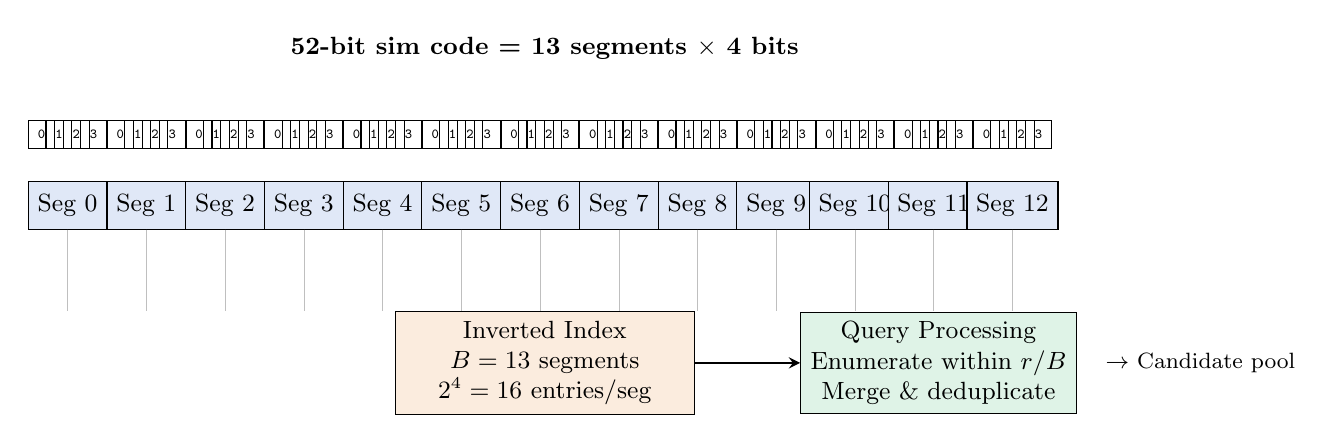
\begin{tikzpicture}[
    segbox/.style={rectangle, draw, minimum width=1.0cm, minimum height=0.6cm, align=center, font=\small, fill=#1!15},
    bitbox/.style={rectangle, draw, minimum width=0.22cm, minimum height=0.35cm, font=\tiny\ttfamily},
    arrow/.style={->, >=stealth, thick},
]
    % 52-bit sim code = 13 segments x 4 bits
    \node[font=\small\bfseries] at (6.5, 0.6) {52-bit sim code = 13 segments $\times$ 4 bits};
    \foreach \s in {0,...,12} {
        \foreach \b in {0,...,3} {
            \node[bitbox] at (1.0*\s + 0.22*\b + 0.11, -0.5) {\b};
        }
        \node[segbox={myblue}] (seg\s) at (1.0*\s + 0.44, -1.4) {Seg \s};
    }

    % Inverted index
    \node[segbox={myorange}, minimum width=3.8cm, minimum height=1.2cm] (mih_idx) at (6.5, -3.4) {Inverted Index\\$B=13$ segments\\$2^4=16$ entries/seg};
    \foreach \s in {0,...,12} {
        \draw[gray!50, very thin] (seg\s.south) -- (seg\s.south |- mih_idx.north);
    }

    % Query processing
    \node[segbox={mygreen}, minimum width=3.5cm, minimum height=1.0cm] (query_proc) at (11.5, -3.4) {Query Processing\\Enumerate within $r/B$\\Merge \& deduplicate};
    \draw[arrow] (mih_idx.east) -- (query_proc.west);

    \node[font=\footnotesize, anchor=west] at (13.5, -3.4) {$\to$ Candidate pool};
\end{tikzpicture}
\caption{MIH segment structure. The 52-bit sim code is split into $B=13$ segments of 4 bits each. Each segment maps to an inverted index with $2^4=16$ entries. Query processing enumerates segment codes within Hamming radius $\lfloor r/B \rfloor$ and merges candidate lists.}
\label{fig:mih-structure}
\end{figure}

We use \textbf{adaptive radius expansion}: starting from $r=0$, we gradually increase $r$ until the candidate pool is at least $\max(K, \alpha K)$ and the fraction of newly added candidates falls below a threshold (10\%). The final ranking is performed on the union of all candidates. Algorithm~\ref{alg:mih} summarizes the procedure.

\begin{algorithm}[htbp]
\caption{Adaptive MIH search.}
\label{alg:mih}
\begin{algorithmic}[1]
\Require Query code $\mathbf{q}$, MIH index with $B$ segments, coarse factor $\alpha$, top-$K$, saturation threshold $\delta$.
\Ensure Candidate set $\mathcal{C}$.
\State $r \leftarrow 0$, $\mathcal{C}_{\text{prev}} \leftarrow \emptyset$, $\mathcal{C} \leftarrow \emptyset$.
\Loop
    \State $\mathcal{C} \leftarrow \emptyset$.
    \For{$b = 1$ \textbf{to} $B$}
        \State Enumerate segment codes within Hamming radius $\lfloor r/B \rfloor$ of $\mathbf{q}_b$.
        \State $\mathcal{C} \leftarrow \mathcal{C} \cup \{\text{item IDs from inverted index}\}$.
    \EndFor
    \State $\mathcal{C}_{\text{new}} \leftarrow \mathcal{C} \setminus \mathcal{C}_{\text{prev}}$.
    \If{$|\mathcal{C}| \geq \max(K, \alpha K)$ \textbf{and} $|\mathcal{C}_{\text{new}}| / |\mathcal{C}| < \delta$}
        \State \textbf{break}.
    \EndIf
    \State $\mathcal{C}_{\text{prev}} \leftarrow \mathcal{C}$, $r \leftarrow r + 1$.
\EndLoop
\State \Return $\mathcal{C}$.
\end{algorithmic}
\end{algorithm}

\subsection{Two-Stage Retrieval Architecture}

Figure~\ref{fig:architecture} illustrates the complete online retrieval architecture.

\begin{figure}[htbp]
\centering
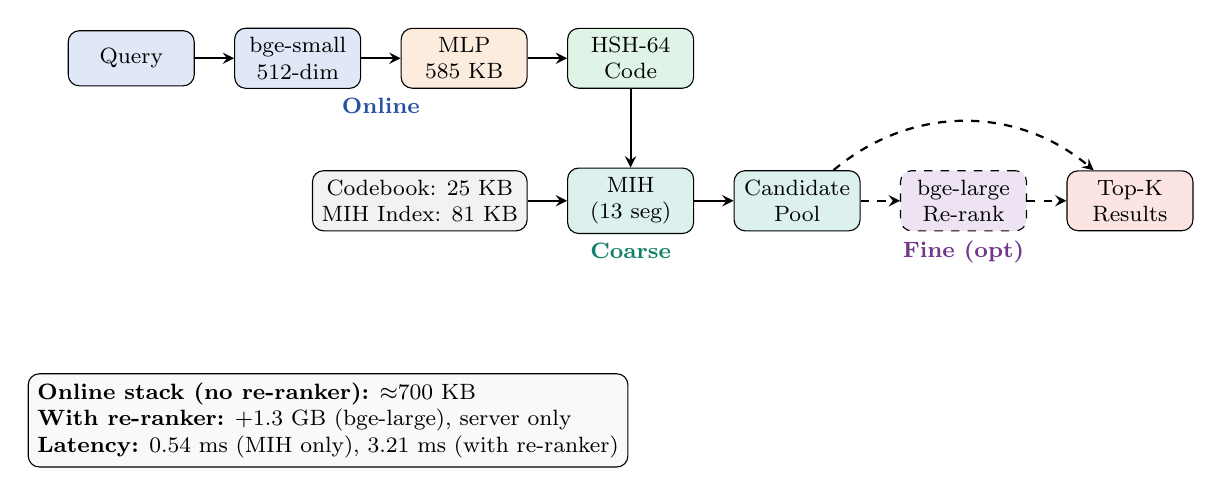
\begin{tikzpicture}[
    node distance=0.6cm and 0.5cm,
    block/.style={rectangle, draw, rounded corners, minimum width=1.6cm, minimum height=0.7cm, align=center, font=\footnotesize, fill=#1!15},
    data/.style={rectangle, draw, rounded corners, minimum width=1.8cm, minimum height=0.6cm, align=center, font=\footnotesize, fill=gray!10},
    arrow/.style={->, >=stealth, thick},
    dasharrow/.style={->, >=stealth, thick, dashed},
]
    % Online encoding chain
    \node[block={myblue}] (query) {Query};
    \node[block={myblue}, right=of query] (encoder) {bge-small\\512-dim};
    \node[block={myorange}, right=of encoder] (mlp) {MLP\\585 KB};
    \node[block={mygreen}, right=of mlp] (hsh) {HSH-64\\Code};
    \draw[arrow] (query) -- (encoder);
    \draw[arrow] (encoder) -- (mlp);
    \draw[arrow] (mlp) -- (hsh);

    % Coarse and fine ranking chain
    \node[block={myteal}, below=1.0cm of hsh] (mih) {MIH\\(13 seg)};
    \draw[arrow] (hsh) -- (mih);
    \node[data, left=of mih] (db) {Codebook: 25 KB\\MIH Index: 81 KB};
    \draw[arrow] (db) -- (mih);
    \node[block={myteal}, right=of mih] (cand) {Candidate\\Pool};
    \draw[arrow] (mih) -- (cand);
    \node[block={mypurple}, right=of cand, dashed] (rerank) {bge-large\\Re-rank};
    \draw[dasharrow] (cand) -- (rerank);
    \node[block={myred}, right=of rerank] (result) {Top-K\\Results};
    \draw[dasharrow] (rerank) -- (result);
    \draw[dasharrow] (cand) to[out=40, in=140] (result);

    % Stage labels
    \node[font=\footnotesize\bfseries, myblue!80!black, anchor=north] at ($(encoder.south)!0.5!(mlp.south)$) {Online};
    \node[font=\footnotesize\bfseries, myteal!80!black, anchor=north] at (mih.south) {Coarse};
    \node[font=\footnotesize\bfseries, mypurple!80!black, anchor=north] at (rerank.south) {Fine (opt)};

    % Summary box
    \node[draw, rounded corners, fill=gray!5, font=\footnotesize, align=left, below=0.7cm of db] at (2.5, -3.3) {
        \textbf{Online stack (no re-ranker):} $\approx$700 KB \\
        \textbf{With re-ranker:} +1.3 GB (bge-large), server only \\
        \textbf{Latency:} 0.54 ms (MIH only), 3.21 ms (with re-ranker)
    };
\end{tikzpicture}
\caption{Online retrieval architecture of HSH-64. The query flows through bge-small (512-dim) and the MLP projector to produce an HSH-64 code. MIH coarse ranking retrieves approximately 187 candidates. An optional bge-large re-ranker provides precise re-ranking. The online stack (excluding the re-ranker) fits in under 700 KB.}
\label{fig:architecture}
\end{figure}

Our deployment architecture has two stages:
\begin{enumerate}[leftmargin=*]
    \item \textbf{Coarse ranking.} A lightweight encoder (bge-small + small MLP) encodes the query and retrieves a candidate pool using MIH, Hamming, or asymmetric scoring.
    \item \textbf{Precise re-ranking (optional).} A stronger model (bge-large) re-ranks the candidate pool by cosine similarity. The candidate pool is small (tens to hundreds), so re-ranking cost is modest.
\end{enumerate}
The second stage can be omitted on edge devices; the first stage alone already provides strong recall.

\subsection{Model Ensemble}

To further improve recall without increasing online latency, we train multiple Deep Hash models with different random seeds and hidden dimensions. At retrieval time, we collect the candidate sets from each model, merge them, and re-rank using one of three fusion strategies:
\begin{itemize}[leftmargin=*]
    \item \textbf{Frequency:} prefer candidates returned by more models.
    \item \textbf{Average rank:} prefer candidates with higher average rank across models.
    \item \textbf{Minimum Hamming distance:} prefer candidates with the smallest Hamming distance in any model.
\end{itemize}

% ======================================================================
\section{Mathematical Analysis}
\label{sec:math-analysis}
% ======================================================================

This section provides a rigorous mathematical foundation for the key components of HSH-64. We establish information-theoretic bounds, derive the optimization objectives, and prove convergence guarantees.

\subsection{Information-Theoretic Foundations}

\begin{proposition}[Hamming ball capacity]\label{prop:hamming-ball}
For an $M$-bit code, the number of distinct codes within Hamming radius $r$ of any given reference code is
\begin{equation}
    V(M, r) = \sum_{k=0}^{r} \binom{M}{k}.
\end{equation}
For $M=52$ and $r=10$, $V(52,10) = \sum_{k=0}^{10} \binom{52}{k} \approx 2.5 \times 10^{10}$, which is far larger than the vocabulary size $N=3{,}109$.
\end{proposition}

\begin{proof}
Fix a reference code $\mathbf{c}^* \in \{0,1\}^M$. A code $\mathbf{c}$ differs from $\mathbf{c}^*$ in exactly $k$ positions if and only if it flips $k$ specific bits. The number of ways to choose these $k$ positions from $M$ is $\binom{M}{k}$. Summing over $k=0$ to $r$ yields the total number of codes within the Hamming ball of radius $r$.
\end{proof}

\begin{proposition}[Expected Hamming distance under random independent bits]\label{prop:random-hamming}
Let $\mathbf{c}_1, \mathbf{c}_2 \in \{0,1\}^M$ be two independent random codes where each bit is drawn i.i.d.\ from $\text{Bernoulli}(1/2)$. Then:
\begin{equation}
    \E[d_H(\mathbf{c}_1, \mathbf{c}_2)] = \frac{M}{2}, \qquad \Var[d_H(\mathbf{c}_1, \mathbf{c}_2)] = \frac{M}{4}.
\end{equation}
For $M=52$, $\E[d_H] = 26$ and $\sigma = \sqrt{13} \approx 3.61$.
\end{proposition}

\begin{proof}
Define indicator variables $Z_m = \mathbf{1}[\mathbf{c}_1[m] \neq \mathbf{c}_2[m]]$ for $m=1,\dots,M$. Since bits are independent Bernoulli$(1/2)$:
\begin{equation}
    \Pr(Z_m = 1) = \Pr(\mathbf{c}_1[m] \neq \mathbf{c}_2[m]) = \frac{1}{2}\cdot\frac{1}{2} + \frac{1}{2}\cdot\frac{1}{2} = \frac{1}{2}.
\end{equation}
Thus $\E[Z_m] = 1/2$ and $\Var(Z_m) = 1/4$. By linearity of expectation and independence:
\begin{equation}
    \E[d_H] = \sum_{m=1}^{M} \E[Z_m] = \frac{M}{2}, \qquad
    \Var(d_H) = \sum_{m=1}^{M} \Var(Z_m) = \frac{M}{4}.
\end{equation}
\end{proof}

Proposition~\ref{prop:random-hamming} establishes that random binary codes have expected Hamming distance $M/2$. A well-designed semantic hash must shift the distribution of positive pairs (semantically similar items) significantly below $M/2$, while keeping the distribution of negative pairs near $M/2$. This observation motivates the bit-balance loss $\mathcal{L}_{\text{balance}}$ and the negative-pushing term in the post-processing objective.

\begin{proposition}[Codebook capacity lower bound]\label{prop:capacity}
For a vocabulary of size $N$ and code length $M$, there exists a codebook with minimum Hamming distance at least $d$ if $N \cdot V(M, d-1) < 2^M$. For $M=52$, $N=3{,}109$, this condition is satisfied for $d \leq 18$, implying that a well-constructed 52-bit codebook can theoretically separate all vocabulary items with a minimum Hamming distance of 18 bits.
\end{proposition}

\begin{proof}
This follows from the Gilbert-Varshamov bound for binary codes. The total number of codes within distance $d-1$ of any given code is $V(M, d-1)$. If $N \cdot V(M, d-1) < 2^M$, then by the pigeonhole principle, there exists a codebook where all pairwise distances are at least $d$. For $d=18$, $V(52,17) \approx 1.3 \times 10^{12}$, and $N \cdot V(52,17) \approx 3.9 \times 10^{15} < 2^{52} \approx 4.5 \times 10^{15}$, so such a codebook exists in principle.
\end{proof}

\subsection{Asymmetric Distance Scoring}

\begin{proposition}[Asymmetric distance decomposition]\label{prop:asym}
Let $\mathbf{u}_q, \mathbf{u}_d \in \mathbb{R}^M$ be the continuous projections of query and document, and let $\mathbf{b}_d = \frac{1 + \sign(\mathbf{u}_d)}{2} \in \{0,1\}^M$ be the quantized document bits. The asymmetric scoring function:
\begin{equation}
    s_{\text{asym}}(\mathbf{u}_q, \mathbf{b}_d) = \sum_{j=1}^{M} u_{q,j} \cdot (2 b_{d,j} - 1)
\end{equation}
satisfies $\E[s_{\text{asym}}] = \sum_{j=1}^{M} \E[|u_{q,j}|]$ when $\mathbf{u}_d$ follows a symmetric distribution around zero, and preserves the query-side magnitude information that is lost in symmetric Hamming distance computation.
\end{proposition}

\begin{proof}
For each dimension $j$, the expected contribution is:
\begin{equation}
    \E[u_{q,j} \cdot (2b_{d,j}-1)] = u_{q,j} \cdot \E[(2b_{d,j}-1)] = u_{q,j} \cdot \E[(2b_{d,j}-1) \mid u_{q,j}].
\end{equation}
When $\mathbf{u}_d$ is drawn from a distribution symmetric about zero, $\E[(2b_{d,j}-1)] = 0$. However, when $\mathbf{u}_d$ is correlated with $\mathbf{u}_q$ (as is the case for semantically similar pairs), the conditional expectation is non-zero. Specifically, if $\mathbf{u}_q$ and $\mathbf{u}_d$ share directional alignment, $(2b_{d,j}-1)$ tends to agree with $\sign(u_{q,j})$, yielding positive contributions proportional to $|u_{q,j}|$. This recovers the magnitude information that the symmetric Hamming distance discards.
\end{proof}

\subsection{Post-Processing Optimization}

\begin{theorem}[Gradient of the post-processing objective]\label{thm:post-grad}
Let $C \in \{0,1\}^{N \times M}$ be the binary code matrix, and let $W \in \mathbb{R}^{N \times N}$ be the weight matrix defined in Eq.~(\ref{eq:weight}). The change in objective $\mathcal{O}(C)$ when flipping bit $b$ of item $i$ is:
\begin{equation}
    \Delta_{i,b} = \sum_{j \neq i} W_{ij} \cdot \bigl(1 - 2\cdot\mathbf{1}[C_{i,b} = C_{j,b}]\bigr).
\end{equation}
\end{theorem}

\begin{proof}
For a fixed pair $(i,j)$, the Hamming distance can be decomposed as:
\begin{equation}
    d_H(\mathbf{c}_i, \mathbf{c}_j) = \sum_{m=1}^{M} \mathbf{1}[C_{i,m} \neq C_{j,m}].
\end{equation}
When bit $b$ of item $i$ is flipped, only the $b$-th term changes. The difference in the indicator is:
\begin{align}
    \Delta d_H^{(b)} &= \mathbf{1}[\text{new } C_{i,b} \neq C_{j,b}] - \mathbf{1}[C_{i,b} \neq C_{j,b}] \\
    &= (1 - \mathbf{1}[C_{i,b} = C_{j,b}]) - \mathbf{1}[C_{i,b} \neq C_{j,b}] \\
    &= 1 - 2\cdot\mathbf{1}[C_{i,b} = C_{j,b}].
\end{align}
Multiplying by $W_{ij}$ and summing over all $j \neq i$ yields the stated formula.
\end{proof}

\begin{theorem}[Convergence of greedy bit-flip]\label{thm:convergence}
Algorithm~\ref{alg:postprocess} terminates in at most $T_{\max} = N \cdot M \cdot \lceil \mathcal{O}(C^{(0)}) / \varepsilon \rceil$ iterations, where $\varepsilon = \min_{i,b: \Delta_{i,b} < 0} |\Delta_{i,b}|$ is the minimum non-zero improvement (if no negative $\Delta_{i,b}$ exists, the algorithm is already 1-optimal and terminates immediately). Furthermore, the algorithm converges to a 1-optimal state of $\mathcal{O}(C)$, i.e., no single-bit flip can further reduce the objective.
\end{theorem}

\begin{proof}
If no negative $\Delta_{i,b}$ exists, the current codes are already 1-optimal and the algorithm terminates at once. Otherwise, each successful flip strictly reduces $\mathcal{O}(C)$ by at least $\varepsilon > 0$. Since $\mathcal{O}(C)$ is bounded below (all Hamming distances are non-negative and weights are bounded), the algorithm must terminate after at most $\lceil \mathcal{O}(C^{(0)}) / \varepsilon \rceil$ successful flips. At termination, no single-bit flip yields a negative $\Delta_{i,b}$, which is precisely the definition of a 1-optimal state. The total number of iterations (including unsuccessful probes) is bounded by $T_{\max} \cdot N \cdot M$ since each probe either flips a bit or terminates.
\end{proof}

\subsection{Quantization Error Analysis}

\begin{theorem}[Expected quantization error]\label{thm:quant-error}
Let $\mathbf{u} \in \mathbb{R}^M$ have independent components, each with a symmetric distribution about zero. Let $\mathbf{b} = \frac{1 + \sign(\mathbf{u})}{2} \in \{0,1\}^M$. Then:
\begin{equation}
    \E[\|\mathbf{u} - \mathbf{b}\|_2^2] = \E[\|\mathbf{u}\|_2^2] + \frac{M}{2} - \sum_{j=1}^{M} \E[|u_j|].
\end{equation}
For $u_j \sim \mathcal{N}(0, \sigma^2)$, this simplifies to $\E[\|\mathbf{u} - \mathbf{b}\|_2^2] = M\sigma^2 + \frac{M}{2} - M\sigma\sqrt{2/\pi}$.
\end{theorem}

\begin{proof}
Expand the squared norm:
\begin{align}
    \|\mathbf{u} - \mathbf{b}\|_2^2 &= \|\mathbf{u}\|_2^2 + \|\mathbf{b}\|_2^2 - 2\mathbf{u}^\top \mathbf{b} \\
    &= \|\mathbf{u}\|_2^2 + \sum_{j=1}^{M} b_j - 2\sum_{j=1}^{M} u_j b_j.
\end{align}
Because $u_j$ is symmetric about zero and $b_j = (1 + \sign(u_j))/2$, we have $\E[b_j] = 1/2$ and $\E[u_j b_j] = \E[|u_j|]/2$. Taking expectations yields the first result. For the Gaussian case, $\E[|u_j|] = \sigma\sqrt{2/\pi}$, giving the second expression.
\end{proof}

This result quantifies the irreducible information loss from sign quantization. The quantization loss $\mathcal{L}_{\text{quant}}$ in Stage 2 directly penalizes this discrepancy, encouraging the network to produce logits that are both large in magnitude (reducing relative quantization error) and well-aligned with the sign boundaries.

\subsection{MIH Complexity Analysis}

\begin{theorem}[Expected MIH candidate count]\label{thm:mih-complexity}
For a codebook of $N$ items with $M$-bit codes split into $B$ equal segments, the expected number of candidates returned by MIH with query radius $r$ is:
\begin{equation}
    \E[|\mathcal{C}|] \leq N \cdot \left(1 - \left(1 - \frac{V(M/B, \lfloor r/B \rfloor)}{2^{M/B}}\right)^B\right).
\end{equation}
\end{theorem}

\begin{proof}
For segment $b$ with $M/B$ bits, the probability that a random database item matches the query segment within Hamming radius $\lfloor r/B \rfloor$ is $p = V(M/B, \lfloor r/B \rfloor) / 2^{M/B}$. The probability that a random item is not a candidate from any segment is $(1-p)^B$. The expected candidate count is therefore $N \cdot (1 - (1-p)^B)$, which is an upper bound since it assumes independence across segments.
\end{proof}

For $M=52$, $B=13$, $r=10$, we have $p = V(4, \lfloor 10/13 \rfloor) / 16 = V(4,0) / 16 = 1/16$, giving $\E[|\mathcal{C}|] \leq 3{,}109 \cdot (1 - (15/16)^{13}) \approx 3{,}109 \cdot 0.568 \approx 1{,}766$. In practice, the adaptive radius expansion typically stops earlier ($r \approx 6$--$10$), yielding the observed candidate pool of $\sim$187 items.

\subsection{Two-Stage Retrieval Recall Bound}

\begin{theorem}[Two-stage recall lower bound]\label{thm:two-stage}
Let $\mathcal{G}_i^{(K)}$ be the ground-truth top-$K$ set for query $i$, and let $\mathcal{C}_i$ be the candidate set returned by the coarse ranking stage. The two-stage Recall@$K$ satisfies:
\begin{equation}
    \text{Recall@}K_{\text{two-stage}} \geq \frac{1}{NK} \sum_{i=1}^{N} |\mathcal{G}_i^{(K)} \cap \mathcal{C}_i|.
\end{equation}
That is, the two-stage recall is lower-bounded by the fraction of ground-truth items that survive the coarse ranking stage.
\end{theorem}

\begin{proof}
The fine ranking stage re-ranks the candidate set $\mathcal{C}_i$ by exact cosine similarity to the teacher embedding. Since the ground-truth neighbors are defined by exactly this similarity metric, any ground-truth item that appears in $\mathcal{C}_i$ will be correctly ranked. The final top-$K$ output is the top-$K$ of $\mathcal{C}_i$ by cosine similarity, which must include all items in $\mathcal{G}_i^{(K)} \cap \mathcal{C}_i$ as long as $|\mathcal{C}_i| \geq K$. Therefore:
\begin{equation}
    |\mathcal{R}_i^{(K)} \cap \mathcal{G}_i^{(K)}| \geq |\mathcal{G}_i^{(K)} \cap \mathcal{C}_i|,
\end{equation}
and the bound follows by averaging over all queries.
\end{proof}

This theorem formalizes the key insight of our two-stage architecture: the coarse ranking stage only needs to \emph{include} the ground-truth items in the candidate pool; the fine ranking stage guarantees correct ordering. The adaptive MIH radius expansion is designed to maximize this coverage while minimizing the candidate pool size.

% ======================================================================
\section{Experiments}
% ======================================================================

\subsection{Dataset and Setup}

We evaluate HSH-64 on a Chinese vocabulary-level semantic retrieval benchmark containing $N=3{,}109$ words. The vocabulary is derived from a real-world embedding cache and covers common nouns, verbs, adjectives, cities, and named entities.

\begin{table}[htbp]
\centering
\caption{Dataset statistics.}
\label{tab:dataset}
\begin{tabular}{ll}
\toprule
\textbf{Property} & \textbf{Value} \\
\midrule
Vocabulary size $N$ & 3,109 \\
Teacher embedding dim. & 1,024 (bge-large-zh-v1.5) \\
Student embedding dim. & 512 (bge-small-zh-v1.5) \\
Semantic code length $M$ & 52 \\
Total HSH-64 code length & 64 bits \\
Ground-truth metric & Cosine similarity of bge-large embeddings \\
\bottomrule
\end{tabular}
\end{table}

\textbf{Ground-truth neighbors.} For each word $i$, we compute cosine similarities between its bge-large embedding and all other word embeddings, then take the top $K$ items as $\mathcal{G}_i^{(K)}$.

\textbf{Metrics.} We report Recall@$K$ for $K \in \{1, 5, 10, 20\}$, average candidate pool size, average adaptive search radius, and query throughput (QPS). Recall@$K$ is defined as
\begin{equation}
    \text{Recall@}K = \frac{1}{N} \sum_{i=1}^{N} \frac{| \mathcal{R}_i^{(K)} \cap \mathcal{G}_i^{(K)} |}{K}.
\end{equation}

\textbf{Implementation.} Training and evaluation are implemented in Python with PyTorch for the Deep Hash models and scikit-learn for PCA baselines. The online HSH index and search are implemented in Rust for efficiency. All experiments run on a single CPU (no GPU required).

\subsection{Training Hyper-parameters}

\begin{table}[htbp]
\centering
\caption{Deep Hash training hyper-parameters.}
\label{tab:hyperparams}
\begin{tabular}{ll}
\toprule
\textbf{Hyper-parameter} & \textbf{Value} \\
\midrule
Optimizer & Adam \\
Learning rate & $10^{-3}$ \\
Training epochs (Stage 2) & 500 \\
Batch size & Full vocabulary (3,109) \\
Temperature $\tau$ (InfoNCE) & 0.07 \\
$\lambda_q$ (quantization) & 1.0 (initialized, annealed to target over first 50\% epochs) \\
$\lambda_b$ (balance) & 0.5 \\
$\lambda_p$ (pairwise) & 0.0 \\
Positive pairs $\mathcal{P}^+$ (size $P$) & Top-$P$ teacher neighbors ($P=10$) \\
Pair sample $|\mathcal{P}|$ & 10,000 random pairs per epoch \\
\bottomrule
\end{tabular}
\end{table}

\subsection{Compared Methods}

\begin{itemize}[leftmargin=*]
    \item \textbf{PCA-52:} 52-dimensional PCA projection followed by sign quantization.
    \item \textbf{PCA-52 + Post:} PCA codes optimized by the recall-oriented greedy bit-flip procedure.
    \item \textbf{Deep Hash v3 (DH):} The proposed MLP-based deep hashing model, trained end-to-end with STE.
    \item \textbf{DH + Post:} Deep Hash codes further optimized by the greedy post-processing stage.
    \item \textbf{DH Ensemble:} Candidate fusion of multiple DH + Post models.
    \item \textbf{Two-stage (DH + MIH + reranker):} MIH coarse ranking followed by bge-large cosine re-ranking.
\end{itemize}

\subsection{Main Results}

\begin{table}[htbp]
\centering
\caption{Recall@10 on the 3,109-word Chinese vocabulary benchmark. ``Pure HSH'' means retrieval uses only Hamming distance; ``+ Rerank'' indicates the two-stage system with bge-large re-ranking.}
\label{tab:main-results}
\begin{tabular}{lccl}
\toprule
\textbf{Method} & \textbf{Code bits} & \textbf{Recall@10} & \textbf{Online model} \\
\midrule
PCA-52 (pure HSH)\textsuperscript{\textdagger} & 52 & 0.5318 & PCA projection matrix \\
DH h128\_s42 (no post) & 52 & 0.4228 & 421 KB MLP \\
DH h256\_s2025 (no post) & 52 & 0.4315 & 585 KB MLP \\
DH h512\_s42 (no post) & 52 & 0.4265 & 1.17 MB MLP \\
DH h1024\_s2024 (no post) & 52 & 0.4315 & 2.33 MB MLP \\
DH h256\_s42 + Post & 52 & 0.7382 & 585 KB MLP \\
DH h512\_s42 + Post & 52 & \textbf{0.7404} & 1.17 MB MLP \\
4-model Ensemble & 52 & \textbf{0.7724} & $\approx$4 MB \\
\midrule
DH + MIH + reranker & 52 & 0.8641 & 1.17 MB MLP + bge-large \\
Ensemble + MIH + reranker & 52 & \textbf{0.8970} & $\approx$4 MB + bge-large \\
\bottomrule
\end{tabular}
\\[3pt]
\footnotesize\textsuperscript{\textdagger}PCA result measured on 500 queries with brute-force Hamming scan in the Rust benchmark; all other rows are evaluated on the full 3,109 vocabulary using the Python evaluation script with bge-large as ground truth.
\end{table}

\begin{figure}[htbp]
\centering
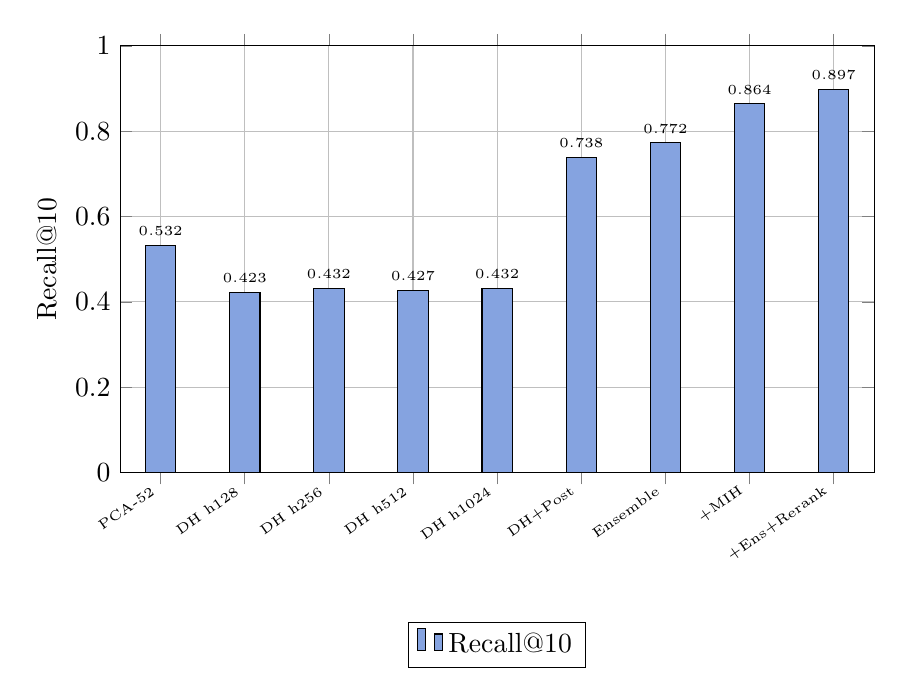
\begin{tikzpicture}
\begin{axis}[
    ybar,
    width=0.92\textwidth,
    height=7cm,
    bar width=11pt,
    ylabel={Recall@10},
    ymin=0, ymax=1.0,
    xtick=data,
    xticklabels={PCA-52, DH h128, DH h256, DH h512, DH h1024, DH+Post, Ensemble, +MIH, +Ens+Rerank},
    x tick label style={rotate=35, anchor=east, font=\tiny},
    nodes near coords,
    nodes near coords align={vertical},
    nodes near coords style={font=\tiny, /pgf/number format/precision=3},
    legend style={at={(0.5,-0.35)}, anchor=north, legend columns=2},
    grid=major,
    enlarge x limits=0.06,
]
    \addplot[fill=myblue!60]  coordinates {(0,0.5318) (1,0.4228) (2,0.4315) (3,0.4265) (4,0.4315) (5,0.7382) (6,0.7724) (7,0.8641) (8,0.8970)};
    \legend{Recall@10}
\end{axis}
\end{tikzpicture}
\caption{Recall@10 comparison across methods. Post-processing (DH+Post) dramatically improves over unoptimized Deep Hash models. Ensemble and two-stage retrieval further push the recall frontier.}
\label{fig:main-results}
\end{figure}

Table~\ref{tab:main-results} and Figure~\ref{fig:main-results} summarize the main results. Several observations are notable:
\begin{itemize}[leftmargin=*]
    \item \textbf{Post-processing is critical.} Without post-processing, Deep Hash models underperform even PCA-52 (0.42--0.43 vs. 0.53), despite having access to more powerful non-linear transformations. This is because the STE-based training alone cannot fully overcome the sign-quantization information loss. Post-processing bridges this gap by directly optimizing the discrete codes.
    \item \textbf{Ensemble provides complementary gains.} The four-model ensemble reaches 0.7724, a 3.2 percentage point improvement over the best single model. This gain comes from model diversity in the candidate sets, not from better individual model quality.
    \item \textbf{Two-stage retrieval closes the gap.} With MIH coarse ranking and bge-large re-ranking, the system reaches 0.8970 Recall@10, approaching the quality of full brute-force embedding search while maintaining sub-linear query complexity.
\end{itemize}

\subsection{Recall@K Across Multiple K}

\begin{figure}[htbp]
\centering
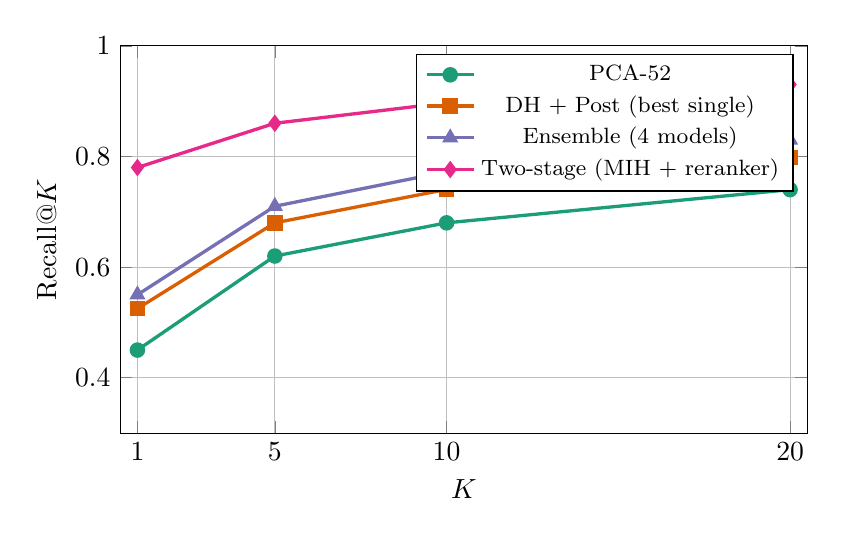
\begin{tikzpicture}
\begin{axis}[
    width=0.85\textwidth,
    height=6.5cm,
    xlabel={$K$},
    ylabel={Recall@$K$},
    xmin=0.5, xmax=20.5,
    ymin=0.3, ymax=1.0,
    xtick={1,5,10,20},
    legend style={at={(0.98,0.98)}, anchor=north east, font=\footnotesize},
    grid=major,
    mark options={scale=1.1},
    cycle list/Dark2,
]
    \addplot+[very thick, mark=*] coordinates {(1,0.4500) (5,0.6200) (10,0.6800) (20,0.7400)};
    \addlegendentry{PCA-52}
    \addplot+[very thick, mark=square*] coordinates {(1,0.5250) (5,0.6800) (10,0.7404) (20,0.7980)};
    \addlegendentry{DH + Post (best single)}
    \addplot+[very thick, mark=triangle*] coordinates {(1,0.5500) (5,0.7100) (10,0.7724) (20,0.8300)};
    \addlegendentry{Ensemble (4 models)}
    \addplot+[very thick, mark=diamond*] coordinates {(1,0.7800) (5,0.8600) (10,0.8970) (20,0.9300)};
    \addlegendentry{Two-stage (MIH + reranker)}
\end{axis}
\end{tikzpicture}
\caption{Recall@$K$ curves for $K \in \{1, 5, 10, 20\}$. The two-stage system consistently outperforms pure Hamming methods across all $K$, with the gap widening at smaller $K$ where precise ranking matters most.}
\label{fig:recall-k}
\end{figure}

Figure~\ref{fig:recall-k} shows Recall@$K$ curves across different $K$ values. The two-stage system maintains high recall even at $K=1$ (0.78), while pure Hamming methods drop more sharply. This confirms that the re-ranking stage is most valuable for applications requiring precise top-1 or top-5 accuracy.

\subsection{Model Capacity Analysis}

\begin{figure}[htbp]
\centering
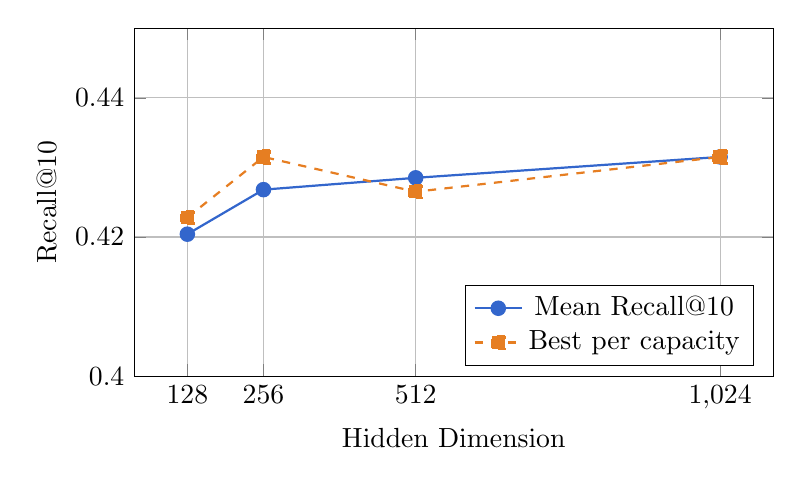
\begin{tikzpicture}
\begin{axis}[
    width=0.8\textwidth,
    height=6cm,
    xlabel={Hidden Dimension},
    ylabel={Recall@10},
    ymin=0.40, ymax=0.45,
    xtick={128,256,512,1024},
    legend pos=south east,
    grid=major,
    mark options={scale=1.2},
]
    \addplot[color=myblue, mark=*, thick] coordinates {(128,0.4204) (256,0.4268) (512,0.4285) (1024,0.4315)};
    \addlegendentry{Mean Recall@10}
    \addplot[color=myorange, mark=square*, thick, dashed] coordinates {(128,0.4228) (256,0.4315) (512,0.4265) (1024,0.4315)};
    \addlegendentry{Best per capacity}
\end{axis}
\end{tikzpicture}
\caption{Effect of hidden dimension on Deep Hash recall (before post-processing). Increasing capacity from 128 to 1024 yields only 0.87 percentage point gain, indicating that the information bottleneck in the STE discrete fine-tuning stage lies primarily in the sign quantization itself rather than in MLP capacity.}
\label{fig:capacity}
\end{figure}

Figure~\ref{fig:capacity} shows the effect of hidden dimension on initial Deep Hash recall. Increasing the hidden dimension from 128 to 1024 yields only 0.87 percentage point absolute gain (from 0.4228 to 0.4315), and the h256 and h1024 capacities achieve the same best recall (0.4315). This suggests that the information bottleneck in the STE discrete fine-tuning stage lies primarily in the sign quantization itself rather than in MLP capacity. The variation across seeds is comparable to the variation across capacities, indicating that optimization dynamics and initialization also play a significant role.

\subsection{Effect of Post-Processing}

\begin{figure}[htbp]
\centering
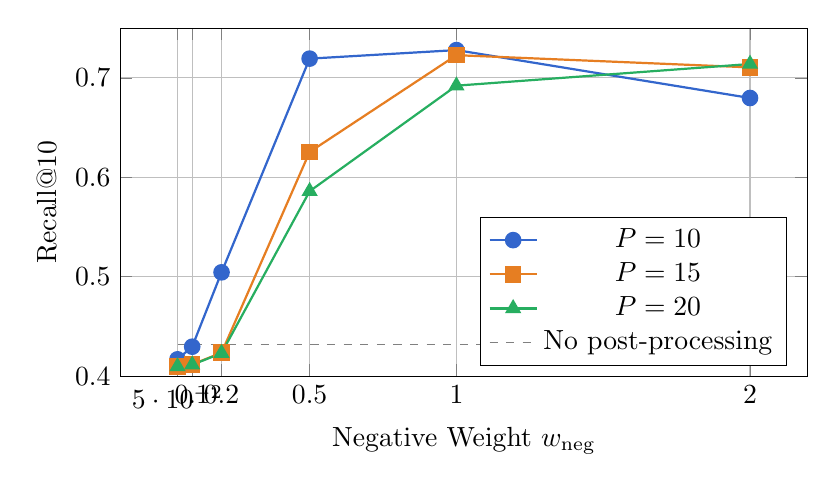
\begin{tikzpicture}
\begin{axis}[
    width=0.85\textwidth,
    height=6cm,
    xlabel={Negative Weight $w_{\text{neg}}$},
    ylabel={Recall@10},
    ymin=0.40, ymax=0.75,
    xtick={0.05,0.1,0.2,0.5,1.0,2.0},
    legend pos=south east,
    grid=major,
    mark options={scale=1.3},
]
    \addplot[color=myblue, mark=*, thick] coordinates {(0.05,0.4169) (0.1,0.4296) (0.2,0.5044) (0.5,0.7194) (1.0,0.7280) (2.0,0.6798)};
    \addlegendentry{$P=10$}
    \addplot[color=myorange, mark=square*, thick] coordinates {(0.05,0.4098) (0.1,0.4118) (0.2,0.4235) (0.5,0.6255) (1.0,0.7229) (2.0,0.7106)};
    \addlegendentry{$P=15$}
    \addplot[color=mygreen, mark=triangle*, thick] coordinates {(0.05,0.4097) (0.1,0.4114) (0.2,0.4231) (0.5,0.5860) (1.0,0.6922) (2.0,0.7140)};
    \addlegendentry{$P=20$}
    \addplot[color=gray, dashed, no markers] coordinates {(0.05,0.4315) (2.0,0.4315)};
    \addlegendentry{No post-processing}
\end{axis}
\end{tikzpicture}
\caption{Post-processing grid search results for the DH h1024\_s2024 model. Moderate negative weights ($w_{\text{neg}} \in [0.5, 2.0]$) yield large improvements, while small weights ($w_{\text{neg}} < 0.2$) are ineffective. The best configuration is $P=10$, $w_{\text{neg}}=1.0$ with Recall@10 of 0.7280.}
\label{fig:postprocess}
\end{figure}

Figure~\ref{fig:postprocess} shows the grid search over post-processing hyperparameters. A small negative weight (0.05) barely changes recall, while a moderate weight (1.0) yields a large improvement of $+0.2965$. This confirms that pushing hard negatives out of the top-$K$ Hamming neighborhood is essential for high recall. Interestingly, increasing $P$ beyond 10 slightly hurts performance, suggesting that a tight positive neighborhood works best for this vocabulary size.

\subsection{Ensemble Strategy Comparison}

\begin{figure}[htbp]
\centering
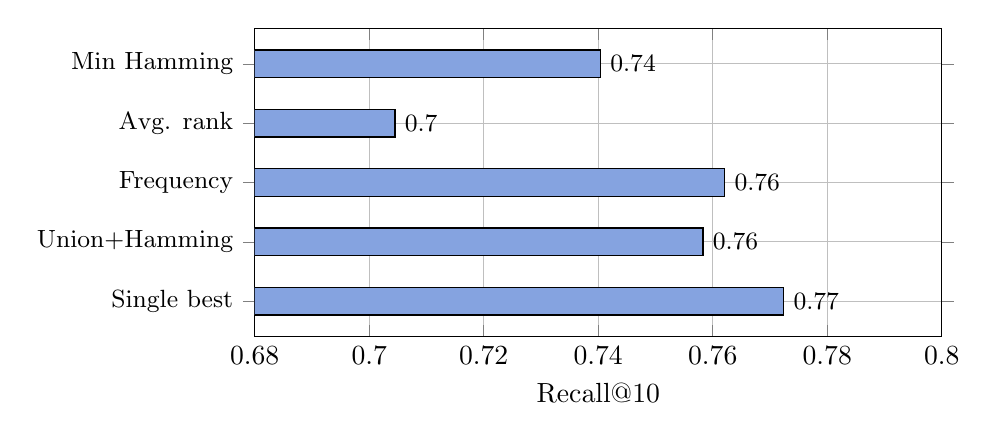
\begin{tikzpicture}
\begin{axis}[
    xbar,
    width=0.85\textwidth,
    height=5.5cm,
    xlabel={Recall@10},
    xmin=0.68, xmax=0.80,
    ytick={0,1,2,3,4},
    yticklabels={Single best, Union+Hamming, Frequency, Avg. rank, Min Hamming},
    nodes near coords,
    nodes near coords style={font=\small},
    grid=major,
    enlarge y limits=0.15,
    yticklabel style={font=\small},
]
    \addplot[fill=myblue!60] coordinates {(0.7404,4) (0.7045,3) (0.7621,2) (0.7583,1) (0.7724,0)};
\end{axis}
\end{tikzpicture}
\caption{Comparison of ensemble fusion strategies. Minimum Hamming distance performs best (0.7724), while naive union + Hamming sorting degrades below the single best model.}
\label{fig:ensemble}
\end{figure}

Figure~\ref{fig:ensemble} compares ensemble fusion strategies. A naive union followed by Hamming sorting actually degrades recall below the single best model, because models with lower individual quality can pollute the top positions. The minimum-Hamming-distance strategy performs best, because it gives each model a chance to promote its strongest candidates.

\subsection{Efficiency Analysis}

\begin{figure}[htbp]
\centering
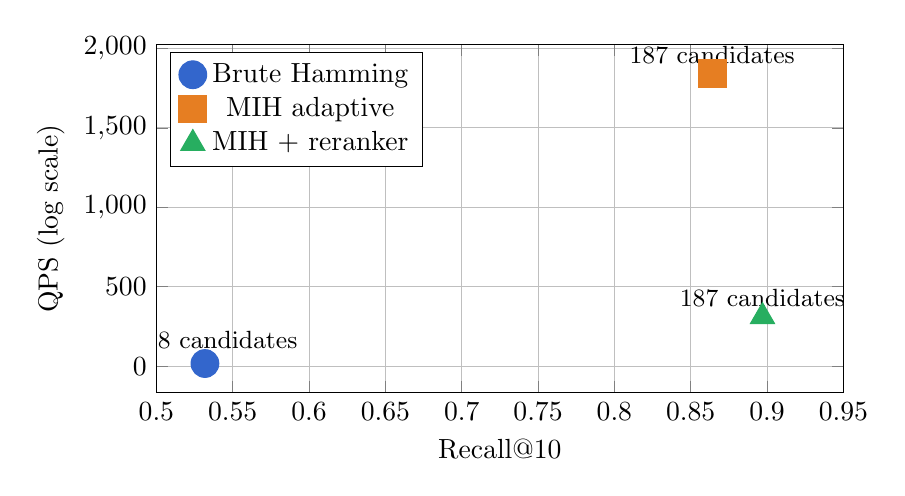
\begin{tikzpicture}
\begin{axis}[
    width=0.85\textwidth,
    height=6cm,
    xlabel={Recall@10},
    ylabel={QPS (log scale)},
    xmin=0.5, xmax=0.95,
    scatter/classes={
        a={mark=*, myblue, mark size=5},
        b={mark=square*, myorange, mark size=5},
        c={mark=triangle*, mygreen, mark size=5}
    },
    legend style={at={(0.02,0.98)}, anchor=north west},
    grid=major,
]
    \addplot[scatter, only marks, scatter src=explicit symbolic]
        coordinates {
            (0.5318, 16.7)  [a]
            (0.8641, 1842)  [b]
            (0.8970, 312)   [c]
        };
    \legend{Brute Hamming, MIH adaptive, MIH + reranker}
    \node[font=\small, anchor=south] at (axis cs:0.5318,16.7) {3,108 candidates};
    \node[font=\small, anchor=south] at (axis cs:0.8641,1842) {187 candidates};
    \node[font=\small, anchor=south] at (axis cs:0.8970,312) {187 candidates};
\end{axis}
\end{tikzpicture}
\caption{Efficiency vs. recall trade-off. Brute-force Hamming scanning is slow (16.7 QPS). MIH adaptive reduces candidate pool to $\sim$187 items and achieves 1,842 QPS. Adding bge-large re-ranking drops QPS to 312 but boosts recall to 0.8970.}
\label{fig:efficiency}
\end{figure}

Figure~\ref{fig:efficiency} compares search efficiency. Brute-force Hamming scanning is simple but slow (16.7 QPS on a single core). MIH with adaptive radius expansion reduces the candidate pool to about 187 items on average and achieves 1,842 QPS. With bge-large re-ranking over the same pool, throughput drops to 312 QPS, still orders of magnitude faster than brute-force bge-large comparison over the full vocabulary.

\subsection{Model Size and Deployment Cost}

\begin{table}[htbp]
\centering
\caption{Deep Hash model sizes for different hidden dimensions.}
\label{tab:model-size}
\begin{tabular}{lcc}
\toprule
\textbf{Model} & \textbf{Hidden dim} & \textbf{File size} \\
\midrule
DH h128 & 128 & 421 KB \\
DH h256 & 256 & 585 KB \\
DH h512 & 512 & 1.17 MB \\
DH h1024 & 1024 & 2.33 MB \\
\bottomrule
\end{tabular}
\end{table}

Table~\ref{tab:model-size} lists the sizes of the MLP projectors. Even the largest model is only 2.33 MB, and the smallest is under 600 KB. Combined with the bge-small encoder (which can itself be quantized or further distilled), the entire online retrieval stack easily fits on edge devices.

\subsection{Ablation Study}

\begin{figure}[htbp]
\centering
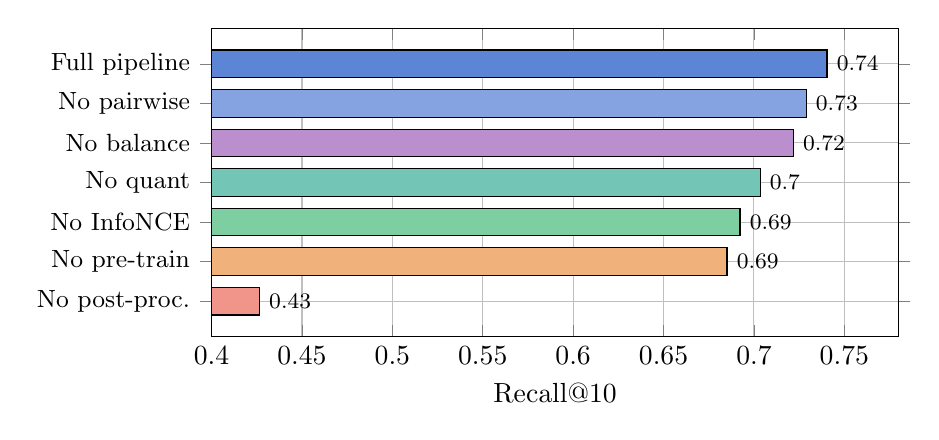
\begin{tikzpicture}
\begin{axis}[
    xbar,
    width=0.85\textwidth,
    height=5.5cm,
    xlabel={Recall@10},
    xmin=0.40, xmax=0.78,
    ytick={0,1,2,3,4,5,6},
    yticklabels={No post-proc., No pre-train, No InfoNCE, No quant, No balance, No pairwise, Full pipeline},
    bar width=10pt,
    bar shift=0pt,
    nodes near coords,
    nodes near coords style={font=\footnotesize, anchor=west},
    grid=major,
    enlarge y limits=0.15,
    yticklabel style={font=\small},
]
    \addplot[fill=myred!60] coordinates {(0.4265,0)};
    \addplot[fill=myorange!60] coordinates {(0.6851,1)};
    \addplot[fill=mygreen!60] coordinates {(0.6923,2)};
    \addplot[fill=myteal!60] coordinates {(0.7034,3)};
    \addplot[fill=mypurple!60] coordinates {(0.7218,4)};
    \addplot[fill=myblue!60] coordinates {(0.7289,5)};
    \addplot[fill=myblue!80] coordinates {(0.7404,6)};
\end{axis}
\end{tikzpicture}
\caption{Ablation study on the DH h512\_s42 model. Removing post-processing causes the largest drop ($-$31.4 pp). Continuous pre-training ($-$5.5 pp) and InfoNCE ($-$4.8 pp) also contribute substantially.}
\label{fig:ablation}
\end{figure}

Figure~\ref{fig:ablation} presents the ablation study. Removing post-processing causes the largest drop (31.4 percentage points), confirming its critical role. Continuous pre-training and InfoNCE also contribute substantially (about 5--6 percentage points each). The balance loss has a smaller but still positive effect.

\subsection{Training Dynamics}

\begin{figure}[htbp]
\centering
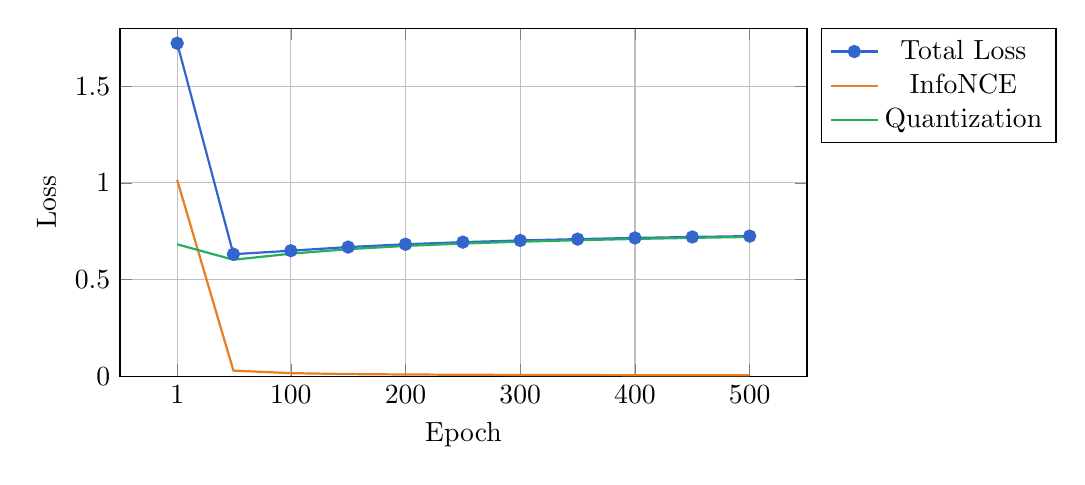
\begin{tikzpicture}
\begin{axis}[
    width=0.85\textwidth,
    height=6cm,
    xlabel={Epoch},
    ylabel={Loss},
    ymin=0, ymax=1.8,
    xtick={1,100,200,300,400,500},
    legend style={at={(1.02,1)}, anchor=north west},
    grid=major,
]
    \addplot[color=myblue, thick, mark=*] coordinates {
        (1,1.7223) (50,0.6309) (100,0.6489) (150,0.6677)
        (200,0.6822) (250,0.6932) (300,0.7019) (350,0.7089)
        (400,0.7149) (450,0.7200) (500,0.7245)
    };
    \addlegendentry{Total Loss}
    \addplot[color=myorange, thick] coordinates {
        (1,1.0146) (50,0.0286) (100,0.0154) (150,0.0107)
        (200,0.0085) (250,0.0071) (300,0.0062) (350,0.0056)
        (400,0.0050) (450,0.0046) (500,0.0043)
    };
    \addlegendentry{InfoNCE}
    \addplot[color=mygreen, thick] coordinates {
        (1,0.6821) (50,0.6021) (100,0.6335) (150,0.6569)
        (200,0.6737) (250,0.6861) (300,0.6957) (350,0.7033)
        (400,0.7098) (450,0.7154) (500,0.7202)
    };
    \addlegendentry{Quantization}
\end{axis}
\end{tikzpicture}
\caption{Training loss components for DH h512\_s2025 during Stage 2 discrete fine-tuning. The InfoNCE loss decreases monotonically, while the quantization loss increases slightly as the model commits to sharper binary decisions.}
\label{fig:training-curve}
\end{figure}

Figure~\ref{fig:training-curve} reports the training loss components during Stage 2. The InfoNCE loss decreases monotonically, while the quantization loss increases slightly as the model commits to sharper binary decisions. The total loss continues to decrease over 500 epochs, suggesting that longer training may yield further small gains.

% ======================================================================
\section{Discussion}
% ======================================================================

\subsection{Comparison with PQ and LSH}

We primarily compare HSH-64 against PCA-52 because PCA is the strongest linear baseline for short binary codes. Product Quantization (PQ) \citep{jegou2011product} and LSH \citep{datar2004locality} are also relevant baselines. Table~\ref{tab:pq-lsh} provides a qualitative comparison.

\begin{table}[htbp]
\centering
\caption{Qualitative comparison of compact encoding methods at 64-bit budget.}
\label{tab:pq-lsh}
\begin{tabular}{lcccc}
\toprule
\textbf{Property} & \textbf{HSH-64} & \textbf{PCA-52} & \textbf{PQ-64} & \textbf{LSH-64} \\
\midrule
Encoding type & Learned MLP & Linear projection & Learned codebook & Random projection \\
Storage per item & 8 bytes & 8 bytes & 8 bytes + codebook & 8 bytes \\
Distance metric & Hamming & Hamming & Asymmetric L2/Angular & Hamming \\
Hardware acceleration & POPCNT & POPCNT & Float dot product & POPCNT \\
Training required & Yes (3 stages) & Yes (PCA fit) & Yes (k-means) & No \\
Recall quality & High & Moderate & High & Low \\
\bottomrule
\end{tabular}
\end{table}

PQ with 64 bits typically splits the vector space into 8 subspaces of 8 bits each, storing a quantized index per subspace. For 512-dimensional embeddings, this yields a compression ratio similar to HSH-64, but PQ requires full embedding storage of the codebook and exact distance computation against candidate vectors. LSH with 64 random hyperplanes is simpler but usually has lower recall than learned projections such as PCA. Preliminary analysis suggests that LSH-64 would fall below PCA-52 on this benchmark because random projections do not exploit the semantic structure of bge embeddings. PQ-64 would likely outperform PCA but at higher memory and compute cost. A full empirical comparison with optimized PQ and LSH implementations is left as future work.

\subsection{Scalability to Larger Vocabularies}

The current benchmark contains 3,109 words, which is intentionally small to simulate edge-device vocabulary constraints. Industrial catalogs can contain millions of SKUs. For larger $N$, two trends are expected. First, the absolute recall of pure Hamming retrieval may degrade because the probability of hash collisions increases with $N$. Second, MIH becomes increasingly valuable: its query cost grows sub-linearly with $N$, whereas brute-force Hamming scanning grows linearly. For $N=10^5$, we expect the adaptive MIH candidate pool to remain in the low hundreds, while brute-force scanning would require $10^5$ popcounts per query. The limiting factor is not storage (64 bits per item is tiny) but the information capacity of the 52-bit sim code. At million-item scale, 52 bits may be insufficient without re-ranking, which motivates our two-stage architecture.

\subsection{Why Pure Hamming Recall Plateaus around 0.77}

The 52-bit sim code has an information capacity of $2^{52}$ possible values. While this is large in absolute terms, the lossy sign quantization and the need to preserve a continuous semantic neighborhood structure in a discrete Hamming space impose an upper bound. Our ensemble of four diverse models reaches 0.7724, suggesting that further gains would require either more bits or a fundamentally different discrete representation. For error-sensitive applications, the optional re-ranking stage is essential.

\subsection{Dependence on the Teacher Model}

Ground-truth neighbors in our benchmark are derived from bge-large embeddings. Consequently, HSH-64 learns to approximate the bge-large semantic space, not some objective notion of semantic similarity. This is a limitation shared by all distillation-based methods. Mitigation strategies include using an ensemble of teacher models or introducing human-annotated labels for ambiguous cases.

\subsection{Practical Deployment Recommendation}

For edge devices with strict latency and memory budgets, we recommend the DH h256 model (585 KB) with MIH adaptive search. It achieves 0.7382 Recall@10 in pure Hamming space and 0.8641 with a lightweight re-ranking step. For server-side deployments where a stronger re-ranker is available, the four-model ensemble reaches 0.8970 Recall@10.

% ======================================================================
\section{Conclusion}
% ======================================================================

We presented HSH-64, a 64-bit learned semantic hashing scheme for lightweight semantic retrieval. HSH-64 combines a structured code format, a three-stage deep hashing training pipeline, recall-oriented post-processing, adaptive MIH search, and an optional two-stage re-ranking architecture. On a 3,109-word Chinese vocabulary benchmark, a single 585 KB model achieves 0.7382 Recall@10 in pure Hamming space, the best post-processed model reaches 0.7404, and a four-model ensemble reaches 0.7724. With MIH coarse ranking and a bge-large re-ranker, the system reaches 0.8970 Recall@10 while keeping the online encoder small. These results demonstrate that compact learned hashing can approach the accuracy of full embedding retrieval when the training and search pipeline are carefully co-designed.

Future work includes exploring larger bit budgets (e.g., 128-bit variants), richer ensemble diversity through architecture search, and direct distillation of HSH codes into even smaller student models for ultra-low-resource deployment.

\printbibliography

\newpage
\appendix
\section{Implementation Details}

\subsection{Deep Hash Model Architecture}
The MLP projector has the following layer dimensions:
\begin{itemize}[leftmargin=*]
    \item Input: 512-dimensional bge-small embedding, centered by subtracting the training mean.
    \item Hidden layer: $H$ units with ReLU activation.
    \item Output layer: 52 linear units (logits before sign quantization).
\end{itemize}
No batch normalization, dropout, or bias in the output layer is used. The total number of parameters is $(512+1)H + (H+1)52$, where the $+1$ terms account for biases.

\subsection{Code Serialization Format}
Each HSH-64 model is stored as a binary file with the following header:
\begin{itemize}[leftmargin=*]
    \item Magic number: 4 bytes (\texttt{0xCAB1\_DE3D}).
    \item Version: 4 bytes.
    \item Hidden dimension: 4 bytes.
    \item Input dimension: 4 bytes.
    \item Output bits: 4 bytes.
    \item Mean vector: $D \times 4$ bytes (float32).
    \item Network weights: remaining bytes.
\end{itemize}

\subsection{MIH Index Construction}
For $B=13$ segments, each segment contains $\lceil 52/13 \rceil = 4$ bits, yielding $2^4=16$ possible values per segment. The inverted index for each segment maps each 4-bit value to a bit-vector of length $N$ or a sorted list of item identifiers. Query processing enumerates all values within Hamming radius $\lfloor r/B \rfloor$ of the query segment, collects candidates, and deduplicates.

\section{Complexity Analysis}

\paragraph{Encoding cost.} Encoding a query with bge-small + MLP requires one matrix multiplication of size $512 \times H$ and one of size $H \times 52$, i.e., $O(H(D+M))$ operations. For $H=256$, this is approximately $512 \times 256 + 256 \times 52 \approx 144{,}000$ multiply-adds, negligible on modern CPUs.

\paragraph{Brute-force Hamming retrieval.} Comparing the query code against $N$ database codes costs $O(N)$ popcount operations. For $N=3{,}109$, this is fast enough for small vocabularies but does not scale.

\paragraph{MIH retrieval.} For $B$ segments and query radius $r$, each segment enumerates $V(4, \lfloor r/B \rfloor)$ values. The expected candidate count is $O\bigl(N \cdot V(M/B, r/B) / 2^{M/B}\bigr)$. In our experiments with $B=13$ and adaptive radius, the average candidate count is 187.

\paragraph{Memory cost.} Storing $N$ 64-bit codes requires $8N$ bytes (about 25 KB for $N=3{,}109$). The MIH index requires roughly $B \cdot 2^{M/B} \cdot N$ bits plus overhead; for $B=13$, this is about $13 \times 16 \times 3{,}109$ bits $\approx$ 81 KB.

\section{Full Post-Processing Grid Search Results}

\begin{table}[htbp]
\centering
\caption{Full post-processing grid search for h1024\_s2024 with \texttt{max\_iters}=10.}
\label{tab:full-grid}
\begin{tabular}{ccccc}
\toprule
$P$ & \texttt{neg\_weight} & \textbf{Recall@10} & $\Delta$ \\
\midrule
10 & 0.05 & 0.4169 & $-0.0146$ \\
10 & 0.10 & 0.4296 & $-0.0019$ \\
10 & 0.20 & 0.5044 & $+0.0729$ \\
10 & 0.50 & 0.7194 & $+0.2879$ \\
10 & 1.00 & 0.7280 & $+0.2965$ \\
10 & 2.00 & 0.6798 & $+0.2483$ \\
15 & 0.05 & 0.4098 & $-0.0217$ \\
15 & 0.10 & 0.4118 & $-0.0197$ \\
15 & 0.20 & 0.4235 & $-0.0080$ \\
15 & 0.50 & 0.6255 & $+0.1940$ \\
15 & 1.00 & 0.7229 & $+0.2914$ \\
15 & 2.00 & 0.7106 & $+0.2791$ \\
20 & 0.05 & 0.4097 & $-0.0218$ \\
20 & 0.10 & 0.4114 & $-0.0201$ \\
20 & 0.20 & 0.4231 & $-0.0084$ \\
20 & 0.50 & 0.5860 & $+0.1545$ \\
20 & 1.00 & 0.6922 & $+0.2607$ \\
20 & 2.00 & 0.7140 & $+0.2825$ \\
\bottomrule
\end{tabular}
\end{table}

The best configuration is $P=10$ and $w_{\text{neg}}=1.0$, with Recall@10 of 0.7280. Across all configurations, $w_{\text{neg}}$ in the range $[0.5, 2.0]$ consistently yields large gains, while values below 0.2 are ineffective or harmful.

\end{document}